\begin{frame}
\frametitle{About This Work...}

\emph{Offline cleaning of RFID trajectory data}~\cite{fazzinga2014offline}\\
B.~Fazzinga, S.~Flesca, F.~Furfaro, F.~Parisi.\\~\\

\begin{itemize}
  \item Published at \emph{SSDBM' 2014}.
  \item A smoothing technique following a two-way filtering scheme that embeds a sampling strategy for efficiently dealing with missing detections.
\end{itemize}

\end{frame}

%------------------------------------------------

\begin{frame}
\frametitle{Motivation}

\begin{itemize}
  \item Pervasive use of RFID devices as a support for object tracking
  \begin{fitemize}
    \item monitoring of people, animals and objects inside museums, schools, hospital etc.
    \item context-aware information.
  \end{fitemize}
  \item There exists ambiguity in the raw RFID data.
  \begin{fitemize}
    \item no one-to-one correspondence between locations and readers, no way to deterministically decide the location given that a set of readers detected an object.
    \item the same location may constrain different reader's detection zones, the same reader may detect different objects at different locations, also false negatives.
  \end{fitemize}
\end{itemize}

\end{frame}

%------------------------------------------------

\begin{frame}
\frametitle{Ambiguity of RFID Data}

\begin{columns}

  \column{0.4\textwidth}
  \begin{figure}[tb]
    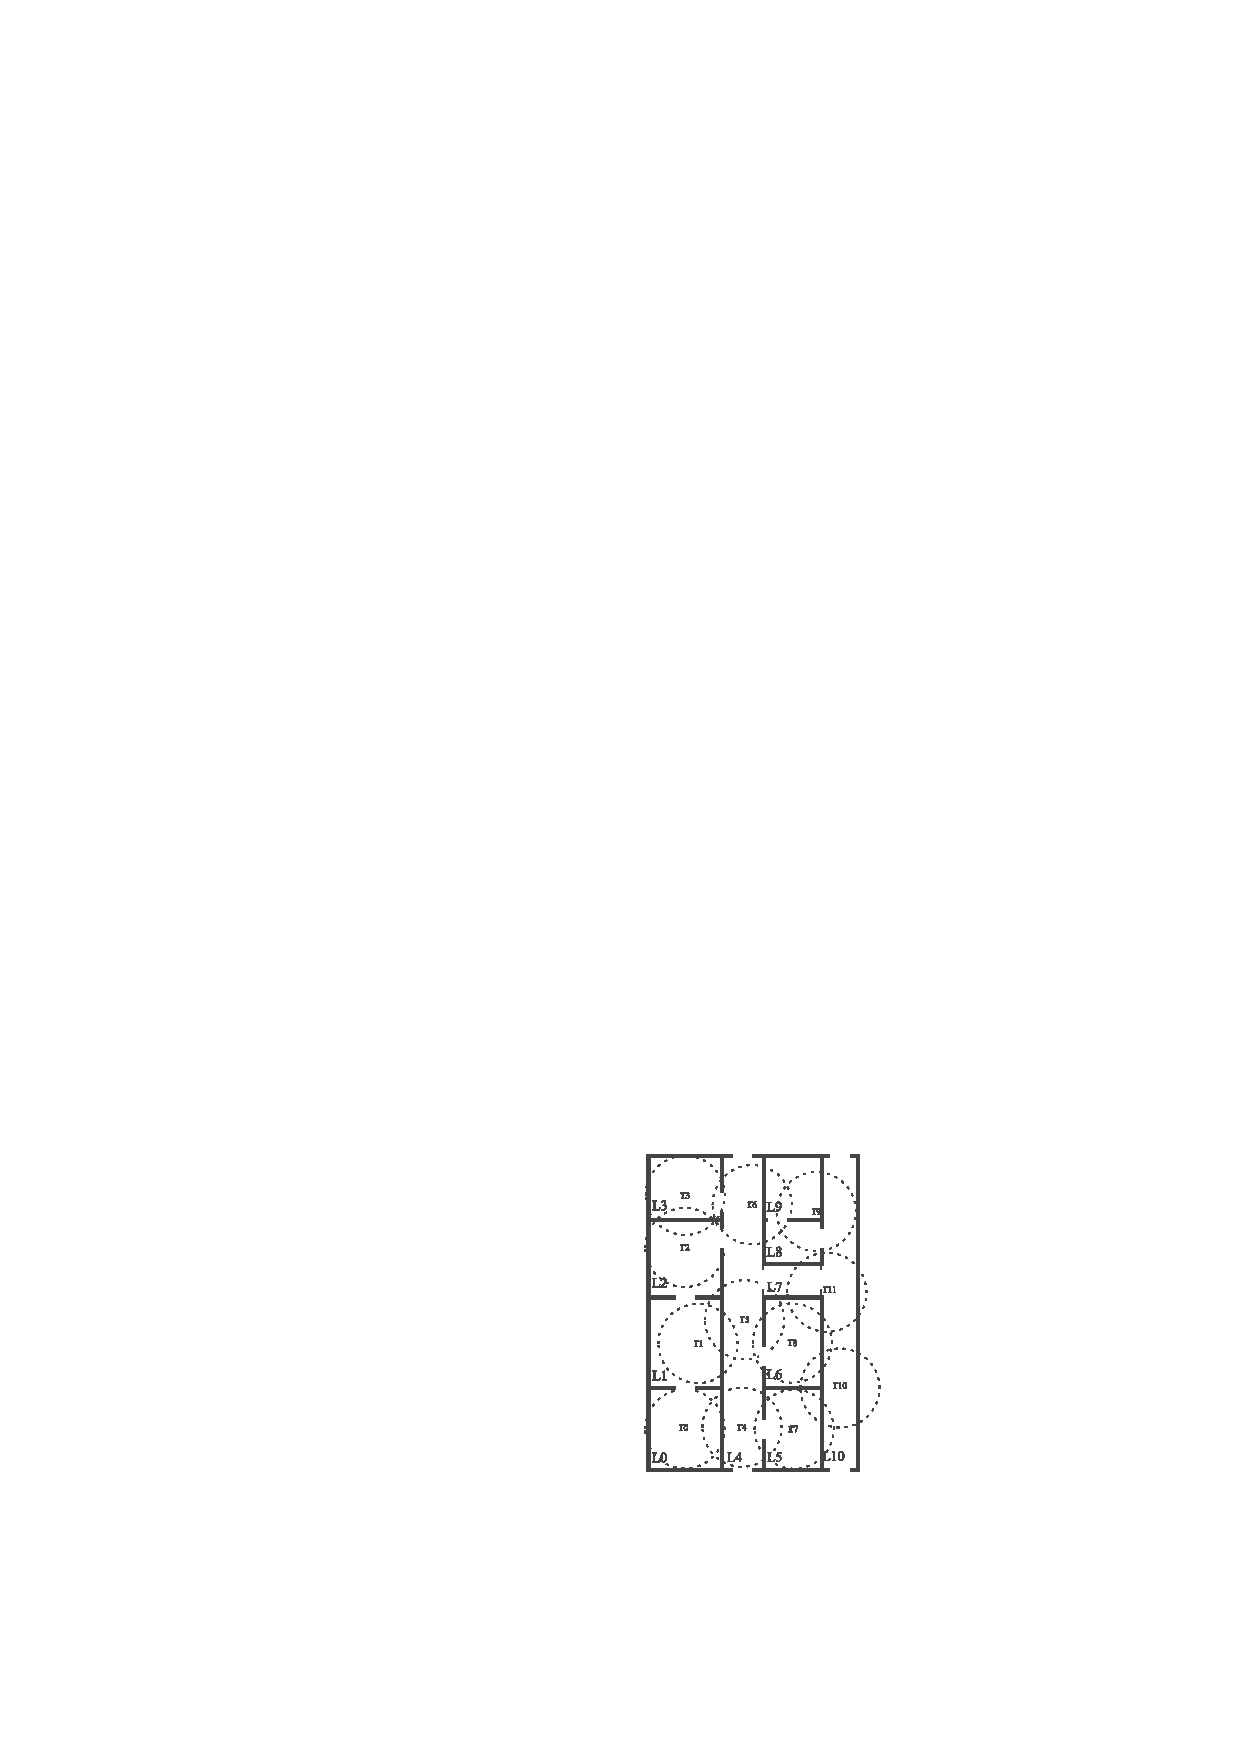
\includegraphics[width=\columnwidth]{figures/3-4/3-4-1.pdf}
  \end{figure}

  \column{0.6\textwidth}
  \begin{example}
    \fsize{
    an object $o$ was detected at some instant by both reader $r_1$ and $r_5$, two locations are possible, $L_1$ and $L_4$. Analogously, if $o$ was detected by $r_3$ only, we cannot conclude that it was surely in $L_3$, as it could be the case that $r_2$ failed to detect it despite it was close enough to its antenna.
    }
  \end{example}

  % \ssize{\textrm{\\this suggests that the association readers/locations can be naturally modeled in probabilistic terms. For instance by a probability distribution $p^a(l|R)$ defined for each location $l$ and set $R$ of readers.}}
  % $p^a(L_1|\{r_1, r_5\}) = p^a(L_4|\{r_1, r_5\}) = 0.5$
  % $p^a(L_0|\{r_0\}) = 1$

\end{columns}

\end{frame}

%------------------------------------------------

\begin{frame}
\frametitle{Ambiguity of RFID Data}

\begin{columns}

  \column{0.4\textwidth}
  \begin{figure}[tb]
    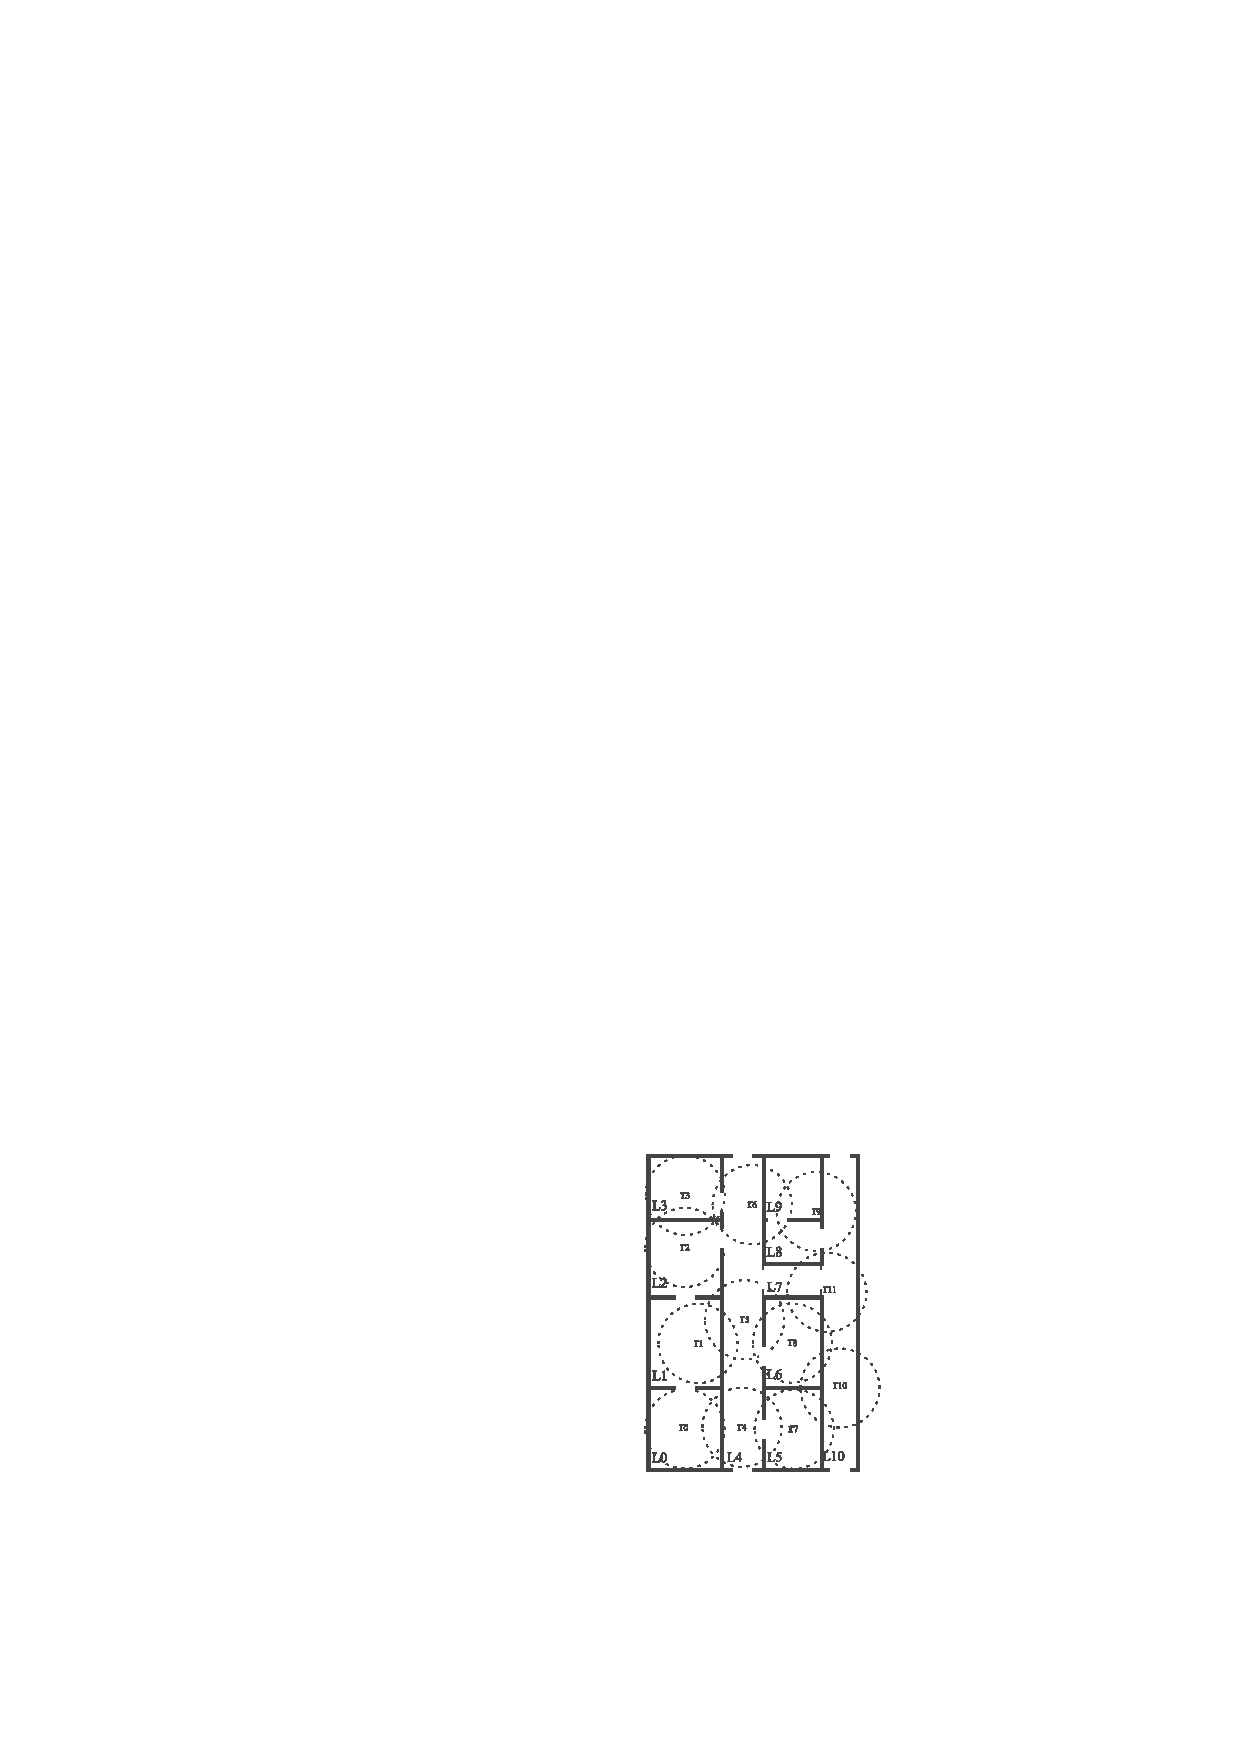
\includegraphics[width=\columnwidth]{figures/3-4/3-4-1.pdf}
  \end{figure}

  \column{0.6\textwidth}
  \begin{figure}[tb]
    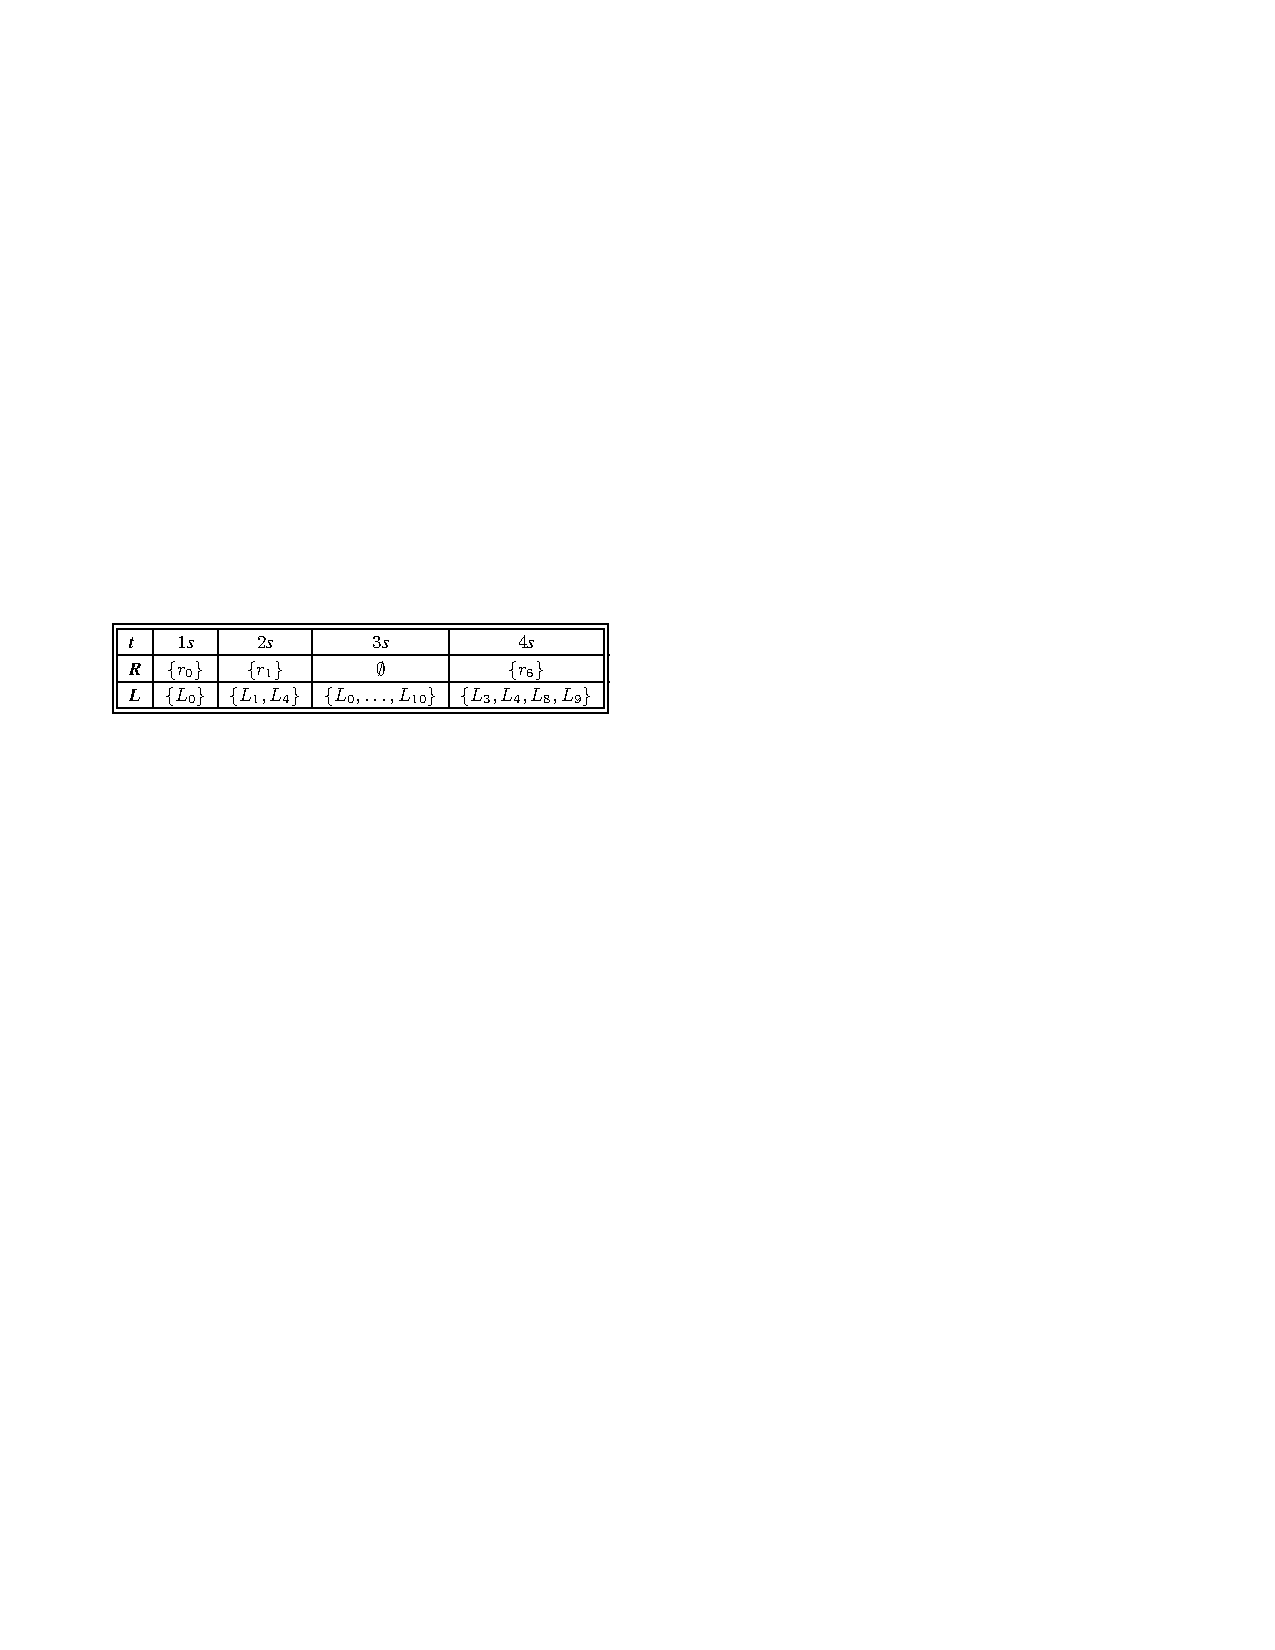
\includegraphics[width=\columnwidth]{figures/3-4/3-4-13.pdf}
  \end{figure}

  \vspace{-10pt}

  \begin{example}
    \ssize{
    $t = 1$: an object detected by $r_0$ is surely at $L_0$ (since the area covered by $r_0$ is totally inside $L_0$)\\
    $t = 2$: an object detected by $r_1$ can be either at $L_1$ or $L_4$ (if object only detected by $r_1$ could also be laid in the area covered by $r_1$ and $r_5$, as $r_5$ may fail to detect the object, the false negative)\\
    $t = 3$: an object detected by no reader can be almost anywhere\\
    $t = 4$: reader $r_6$ covers portions of $L_3, L_4, L_8, L_9$ only.
    }
  \end{example}


\end{columns}

\end{frame}

%------------------------------------------------

\begin{frame}
\frametitle{Ambiguity of RFID Data}

\ssize{\textrm{assume that $o$ is a person, his maximum speed is $v_{max} = 2m/s$. Consider the size of the floor is $15m \times 11m$, re-examine the possible location as follow:}}

\vspace{10pt}

\begin{columns}

  \column{0.3\textwidth}
  \begin{figure}[tb]
    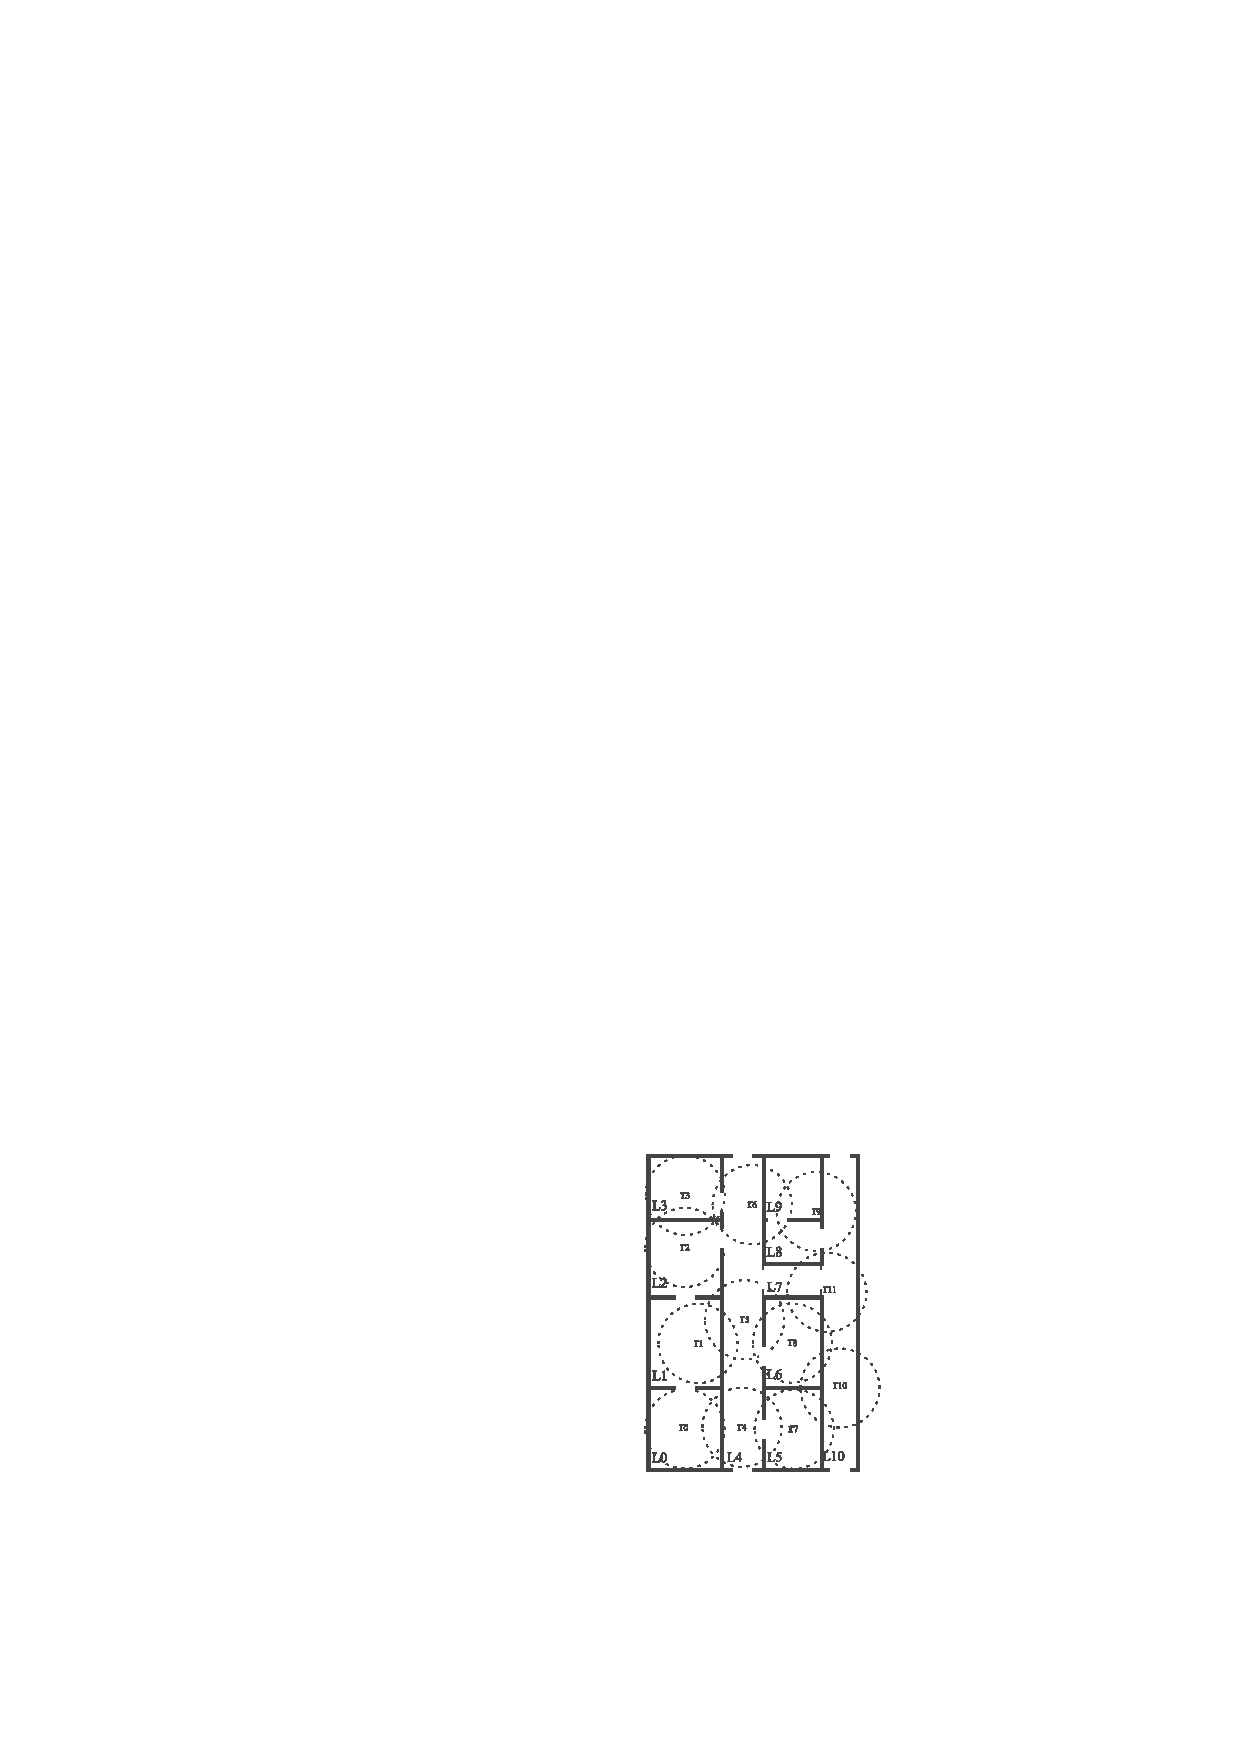
\includegraphics[width=\columnwidth]{figures/3-4/3-4-1.pdf}
  \end{figure}


  \column{0.7\textwidth}
  \ssize{
  A.  As regards $t = 2s$, $o$ must be at $L_1$, as it cannot be at $L_4$. In fact, $o$ was at $L_0$ at $t = 1s$, and the minimum (indoor) distance between $L_0$ and $L_4$ (about 7m) cannot be covered in $1sec$ without exceeding $v_{max}$. \\~\\
  B.  As regards $t = 3s$, now that it has been established that $o$ was at $L_1$ at $t = 2s$, we can restrict the set of possbile locations from $\{ L_1,...,L_{10} \}$ to $\{ L_0, L_1, L_2 \}$ (due to the size of the floor, reaching a room not in this set from any position inside $L_1$ in one second would require a speed greater than $v_{max}$). \\~\\
  C.  As regards $t = 4s$, the only location in $\{ L_3, L_4, L_8, L_9 \}$ (the set of location covered by $r_6$) that can be reached from at least one location in $\{ L_0, L_1, L_2 \}$ (the possible locations at time $t = 3s$, as established at point B) is $L_4$.
  }


\end{columns}

\end{frame}

%------------------------------------------------

\begin{frame}
\frametitle{Ambiguity of RFID Data}

\ssize{\textrm{all the arguments used in Point A,B,C show that the exploiting the correlation with the past positions can reduce (or even eliminate) the uncertainty in determining the position at any time point. Trying to further reduce the uncertainty by exploiting the correlation:}}

\vspace{10pt}

\begin{columns}

  \column{0.3\textwidth}
  \begin{figure}[tb]
    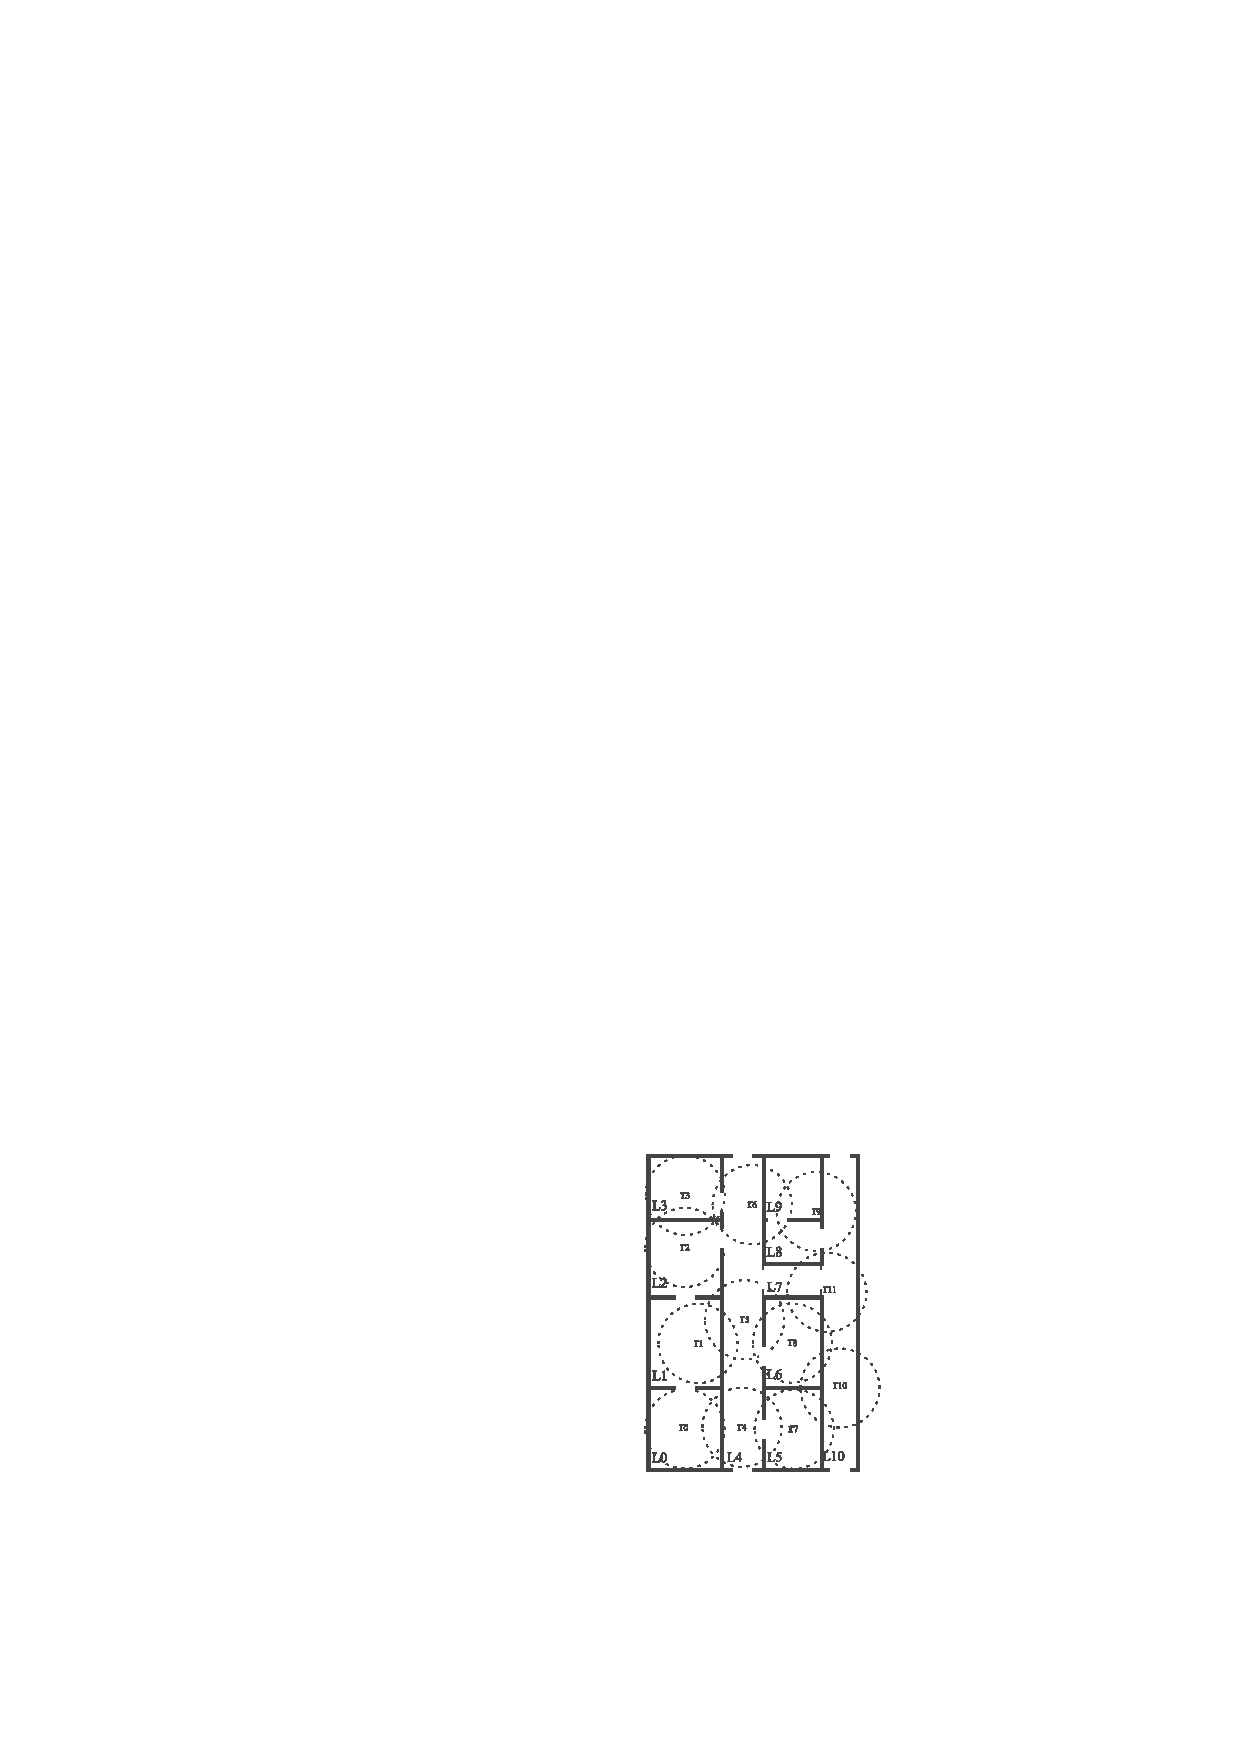
\includegraphics[width=\columnwidth]{figures/3-4/3-4-1.pdf}
  \end{figure}


  \column{0.7\textwidth}
  \ssize{
  D.  Consider $t = 3s$, we have already established that the position of $o$ at the subsequent time point is $L_4$, and that the possible locations for this time point are $L_0, L_1, L_2$. Hence, at $t = 3s$, $o$ must have been at $L_2$, as this is the only among the possible locations for this time point from which $L_4$ can be reached in one second without exceeding $v_{max}$.
  }

  \begin{figure}[tb]
    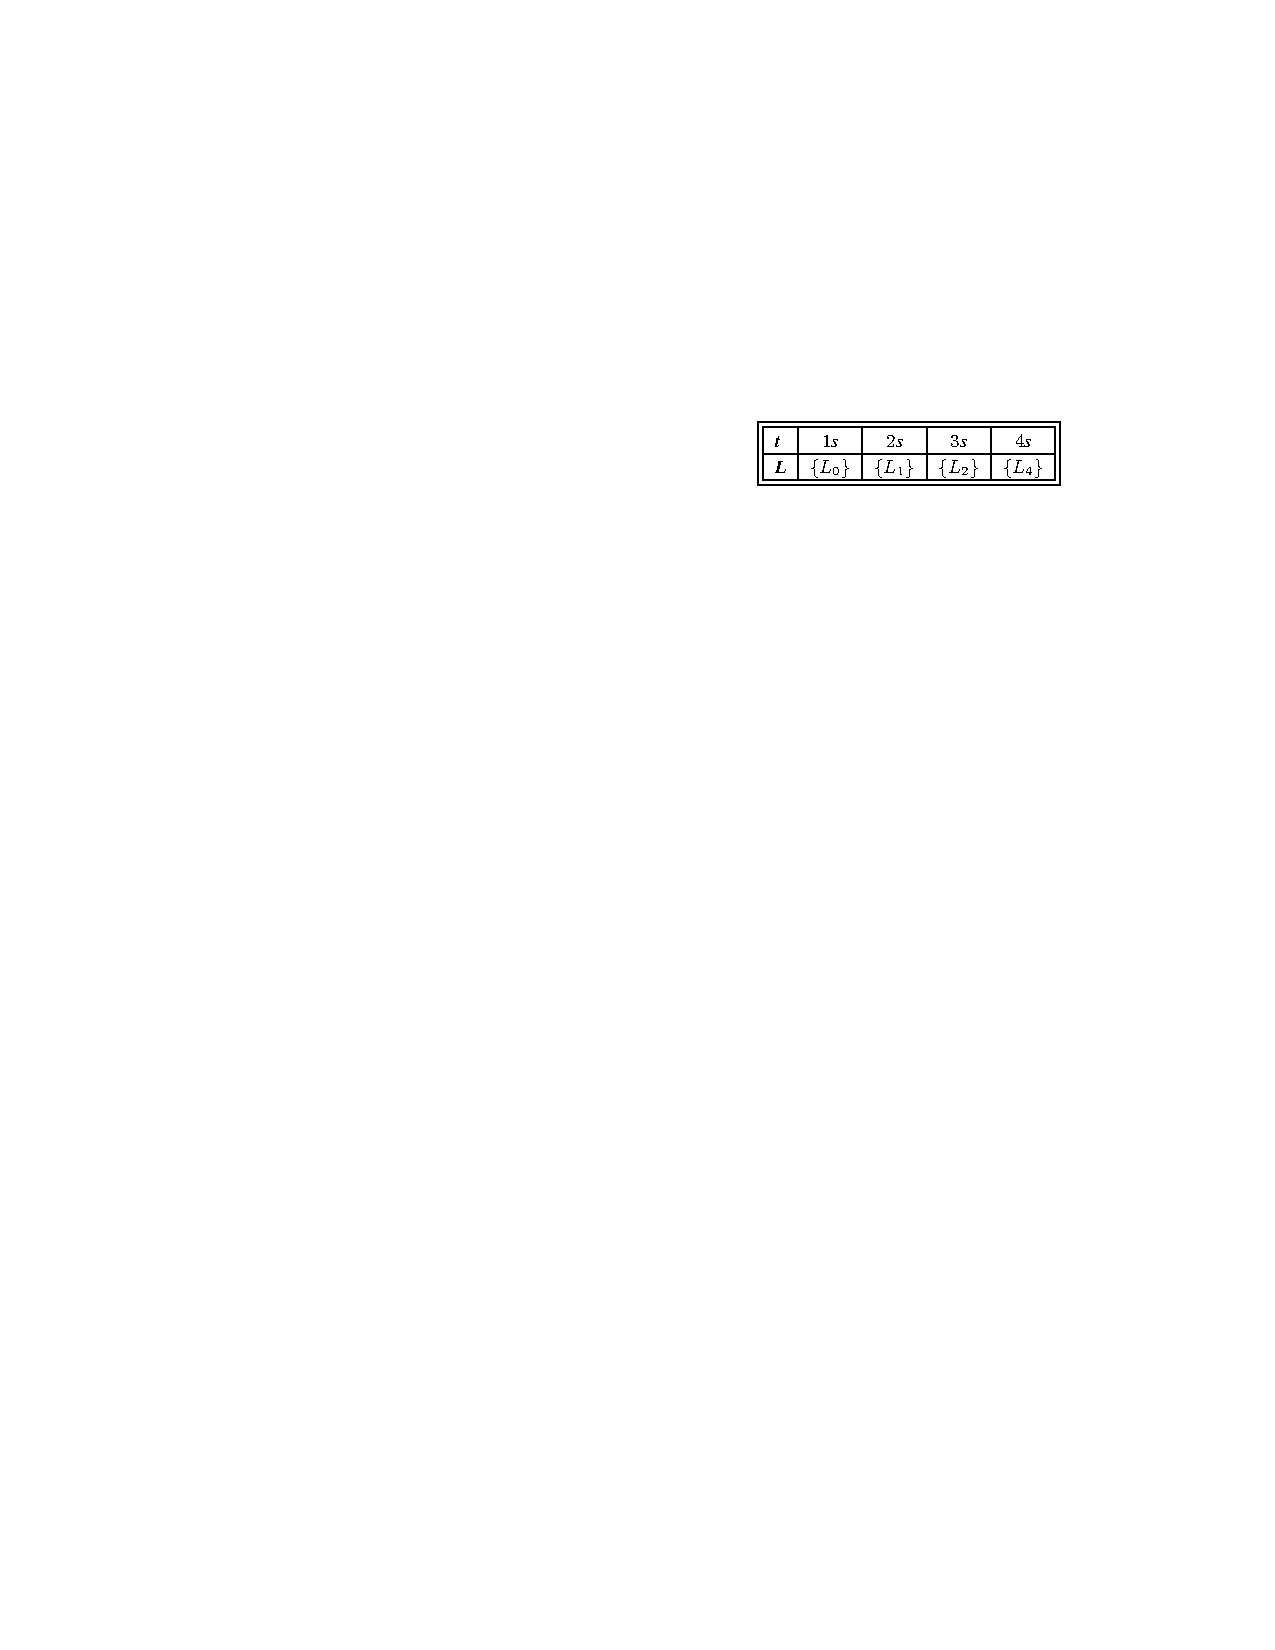
\includegraphics[width=\columnwidth]{figures/3-4/3-4-14.pdf}
  \end{figure}


\end{columns}

\end{frame}

%------------------------------------------------

\begin{frame}
\frametitle{The Problem Setting for This Work}

\fsize{

An instance of \conceptbf{smoothing problem}~\cite{smith2013sequential}: estimating the state of an observed entity at a time point $t \in [1...T]$ on the basis of all the observations over $[1...T]$ in terms of a posterior probability distribution over the possible states.\\~\\

This work proposes a smoothing technique following a two-way-filtering scheme that embeds a sampling strategy for efficiently dealing with missing detections.\\~\\

In the first \emph{forward} phase, time points are processed from the first to the last, and the possible positions at each time point are filtered by taking into account the results of the previous steps.\\~\\

In the \emph{backward} phase, it proceeds from the last to the first time point: for each time point, filter the positions detected as admissible in the forward phase and revise their weights, by checking whether they are a valid position when looking at the results obtained for the future time point.

}

\end{frame}

%------------------------------------------------

\begin{frame}
\frametitle{The Problem Setting for This Work}

\fsize{

The map of the locations is assumed to be partitioned according to a grid, thus the positions to be filtered and weighted at each step of the forward phase are the grid cells compatible with the readers that performed the detection.\\~\\

Thus, the grid cells may result in too many candidate positions, a variant of the cleaning algorithm where missing detections are treated by integrating the grid-based approach with sampling strategy is proposed.\\~\\

At the end of each forward step involving a missing detection, the cells that survived the filtering are further filtered according to a sampling technique, where the probability of a cell to be sampled is an estimate of the probability it would have been assigned if it was considered also in the following phases.

}

\end{frame}

%------------------------------------------------

\begin{frame}
\frametitle{The Preliminaries}

\begin{figure}[tb]
  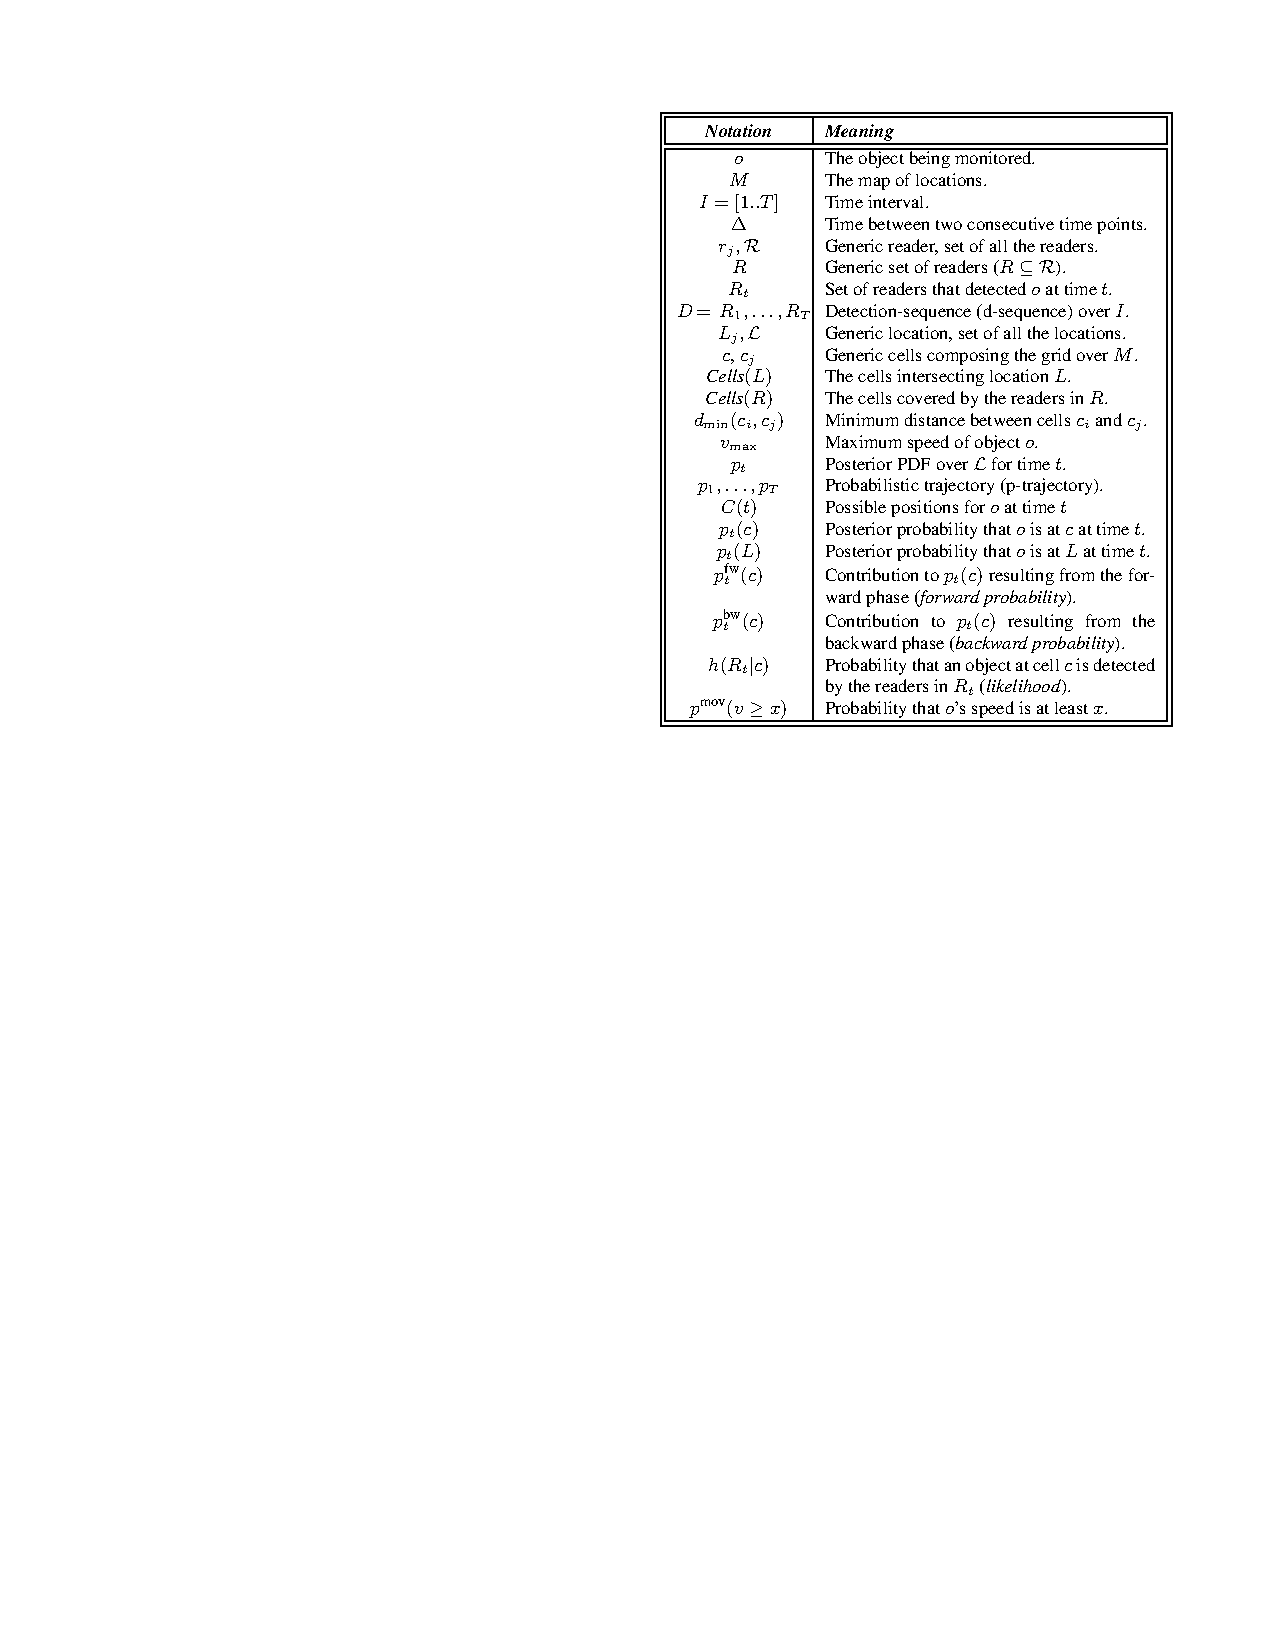
\includegraphics[width=0.55\columnwidth]{figures/3-4/3-4-15.pdf}
\end{figure}

\end{frame}

%------------------------------------------------

\begin{frame}
\frametitle{The Preliminaries}

Assume the set $\mathcal{R} = \{ r_1,...,r_n \}$ of readers, and the set $\mathcal{L} = \{ L_1,...,L_n \}$ of locations on map $M$.\\~\\ \pause

The map of locations is partitioned according to a regular grid, whose generic cell will be denoted as $c$. The set of cells intersecting the area covered by a set $R \in \mathcal{R}$ of readers will be denoted as $Cells(R)$. \\~\\ \pause

A \emph{detection-sequence} (d-sequence for short) $D$ over time interval $I$ is a sequence $R_1,...,R_T$, where $R_t \subset \mathcal{R}$ (with $t \in [1...T]$) is the (possibly empty) set of readers that detected $o$ at time point $t$.

\end{frame}

%------------------------------------------------

\begin{frame}
\frametitle{The Preliminaries}

\begin{problem}[The Cleaning Problem]
  Given a d-sequence $D = R_1,...R_T$, representing the sets of readers that consecutively detected object $o$ while it was moving over the time interval $I = [1...T]$ and over the map $M$, the \emph{cleaning problem} addressed in this work is that of estimating the actual position (at the granularity level of location) of $o$ at each $t \in I$. This will be accomplished by modeling the position of $o$ at $t$ as a random variable over $\mathcal{L}$, and providing a posterior PDF $p_t$ which is conditional to the relevant evidence encoded by the d-sequence $D$. The output of this cleaning task is the sequence $p_1,...p_T$ of these posterior PDFs, and will be called \emph{probabilistic trajectory} (p-trajectory) over time interval $I$.
\end{problem}

\end{frame}

%------------------------------------------------

\begin{frame}
\frametitle{The Cleaning Algorithm}

\begin{block}{A Motion Model for estimating the probability of movements}
  Given two cells $c, c'$, to estimate the probability that object $o$ has reached $c'$ starting from $c$ in a certain amount of time. To this end, we exploit the knowledge of $v_{max}$, and we assume that the possible speeds of $o$ are uniformly distributed over $[0,v_{max}]$. Then, denoting the probability that the speed of $o$ is at least $x$ as $p^{mov}(v \geq x)$, we estimate the probability that $o$ reached $c'$ from $c$ in time $\Delta$ as the probability that $o$ had at least the speed needed to walk through the shortest path from $c$ to $c'$ in time $\Delta$, i.e., $p^{mov} (v \geq d_{min}(c,c')/\Delta)$.
\end{block}

\textit{\textrm{this way, the probability in motion model takes into account both the maximum speed and the topology of the map (that implies the value of $d_{min}$).}}

\end{frame}

%------------------------------------------------

\begin{frame}
\frametitle{The Cleaning Algorithm: Overview}

\begin{columns}

  \column{0.5\textwidth}
  \begin{figure}[tb]
    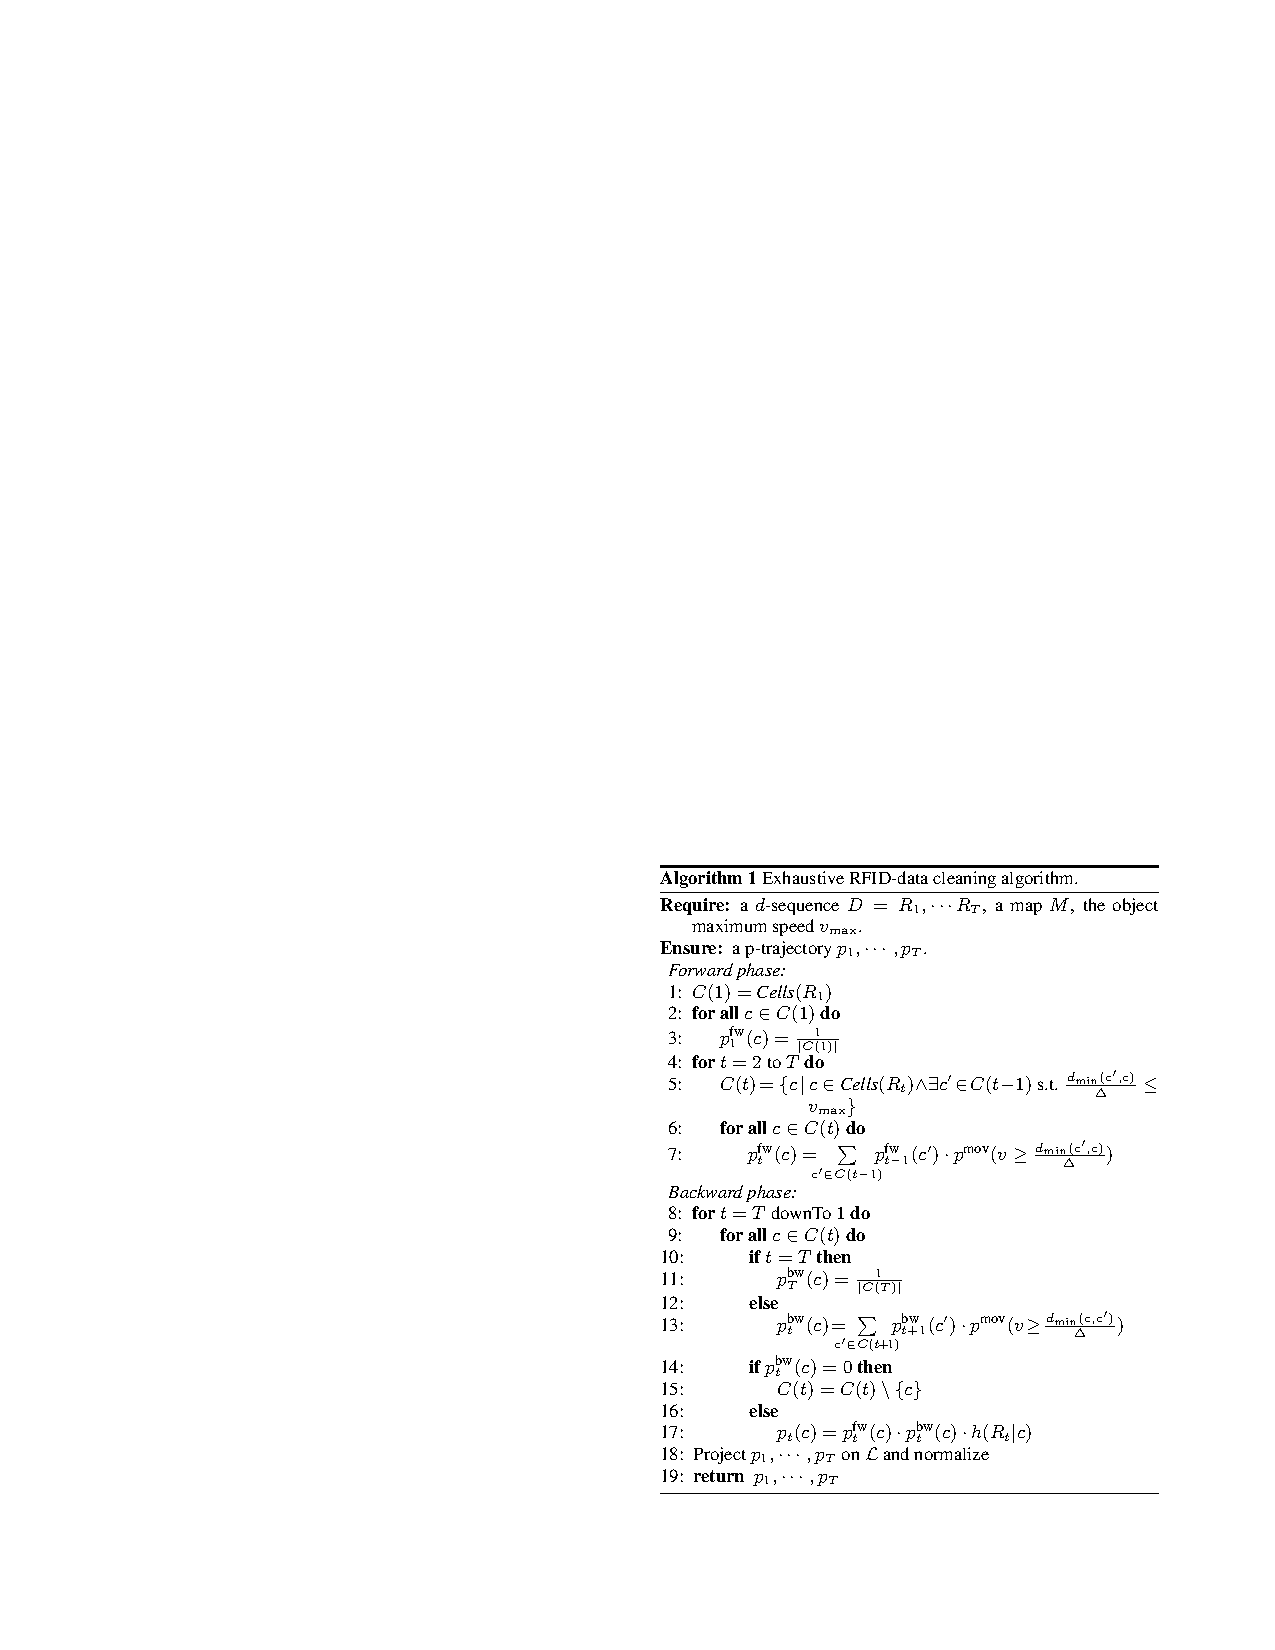
\includegraphics[width=\columnwidth]{figures/3-4/3-4-16.pdf}
  \end{figure}

  \column{0.5\textwidth}
  \begin{sitemize}
    \item consists of the \emph{forward} phase and the \emph{backward} phase.
    \item during the forward phase, the input d-sequence is progressively scanned from the first to the last time point, for each time point $t \in [1...T]$, a set $C(t)$ of cells is determined, meaning the \emph{possible} positions of $o$ at $t$.
    \item ``possible'' means these positions are consistent both with the detections at $t$ itself and with the positions which have been recognized as possible for $o$ at previous time point.
    \item each cell $c$ in $C(t)$ is assigned a \emph{forward probability} $p^{fw}_t(c)$, which represents the probability that $c$ is the position at $t$ (only the past time points have been taken into account), it's evaluated using the motion model.
  \end{sitemize}

\end{columns}

\end{frame}

%------------------------------------------------

\begin{frame}
\frametitle{The Cleaning Algorithm: Overview}

\begin{columns}

  \column{0.5\textwidth}
  \begin{figure}[tb]
    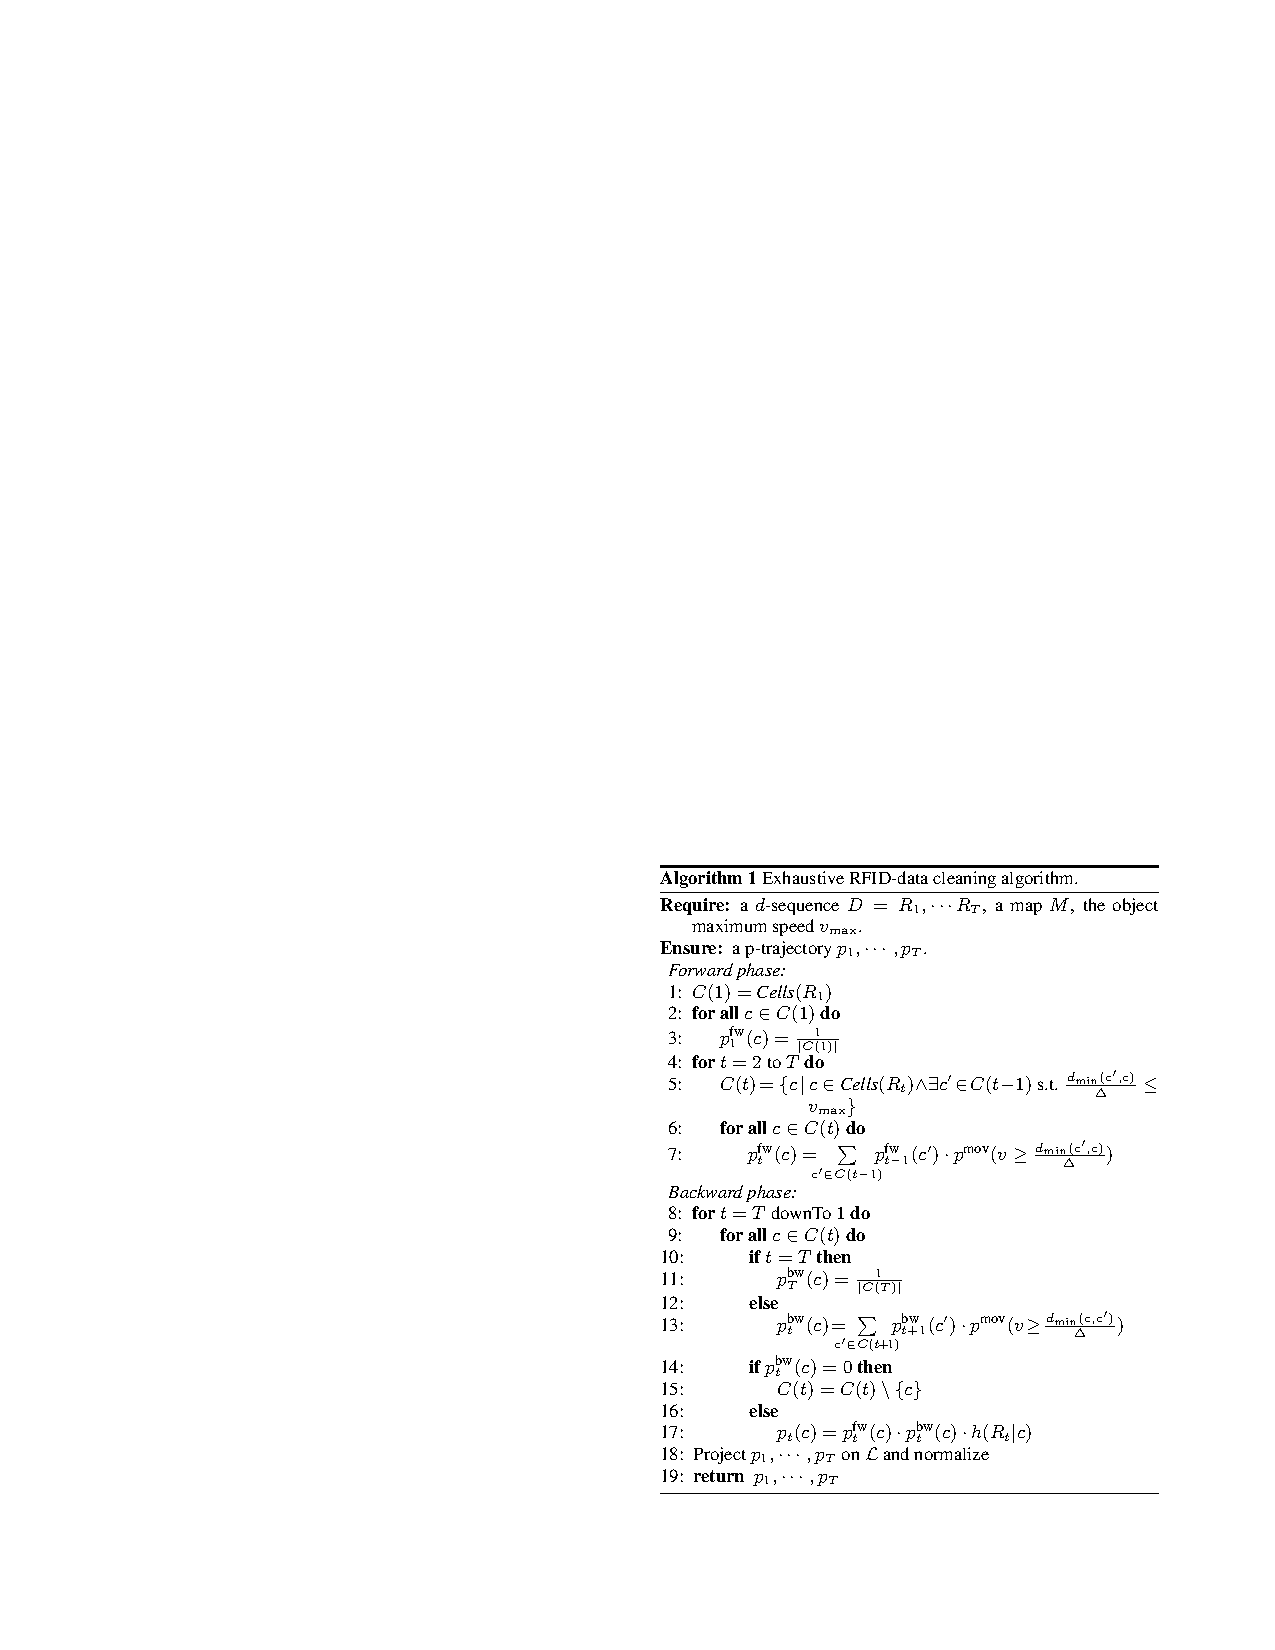
\includegraphics[width=\columnwidth]{figures/3-4/3-4-16.pdf}
  \end{figure}

  \column{0.5\textwidth}
  \begin{sitemize}
    \item the backward phase is analogous to the forward one but processes in inverse order on the result by forward phase.
    \item for each cell in $C(t)$, the \emph{backward probability} $p^{bw}_t(c)$ is computed: it represents the probability that $c$ is the position at $t$, when only the possible positions at time points in $[t+1,T]$ are taken into account.
    \item cells with backward porbability equal to $0$ are removed from $C(t)$, since they are turne out to be inconsistent with the possible positions in $[t+1,T]$.
  \end{sitemize}

\end{columns}

\end{frame}

%------------------------------------------------

\begin{frame}
\frametitle{The Cleaning Algorithm: Overview}

\begin{columns}

  \column{0.5\textwidth}
  \begin{figure}[tb]
    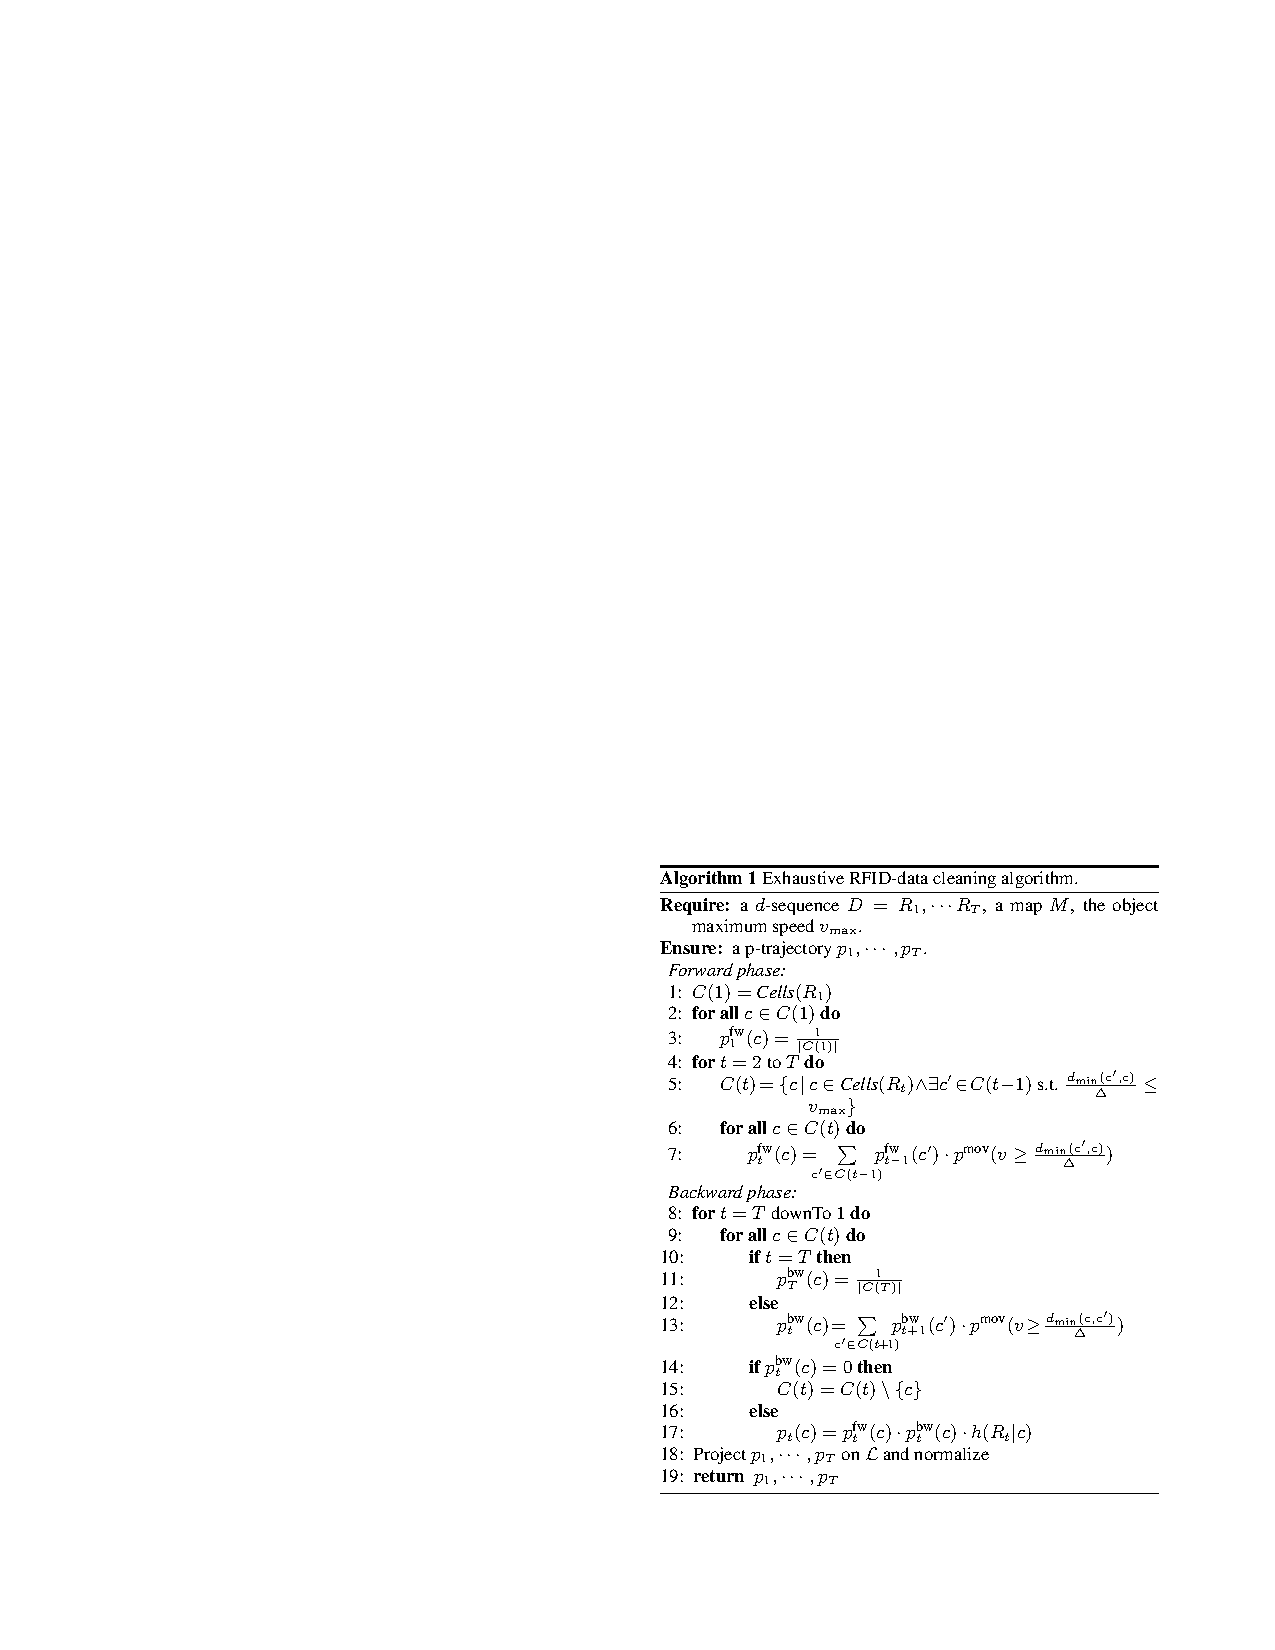
\includegraphics[width=\columnwidth]{figures/3-4/3-4-16.pdf}
  \end{figure}

  \column{0.5\textwidth}
  \begin{sitemize}
    \item at the end of backward phase, for each $t \in [1...T]$ and cell $c \in C(t)$, the posterior probability $p_t(c)$ is finally computed as the product among the following 3 constributions: $p^{fw}_t(c)$, $p^{bw}_t(c)$ and likelihood $h(R_t|c)$ (the probability that $o$ is detected by the reaaders in $R_t$ given that $o$ is at cell $c$).
    \item The so obtained functions $p_1, ..., p_T$ are then projected over the locations and normalized. A probabilistic trajectory where the PDF at each time point is computed by considering the past, the present and the future readings.
  \end{sitemize}

\end{columns}

\end{frame}

%------------------------------------------------

\begin{frame}
\frametitle{The Cleaning Algorithm: Overview}

The above-sketch approach may turn out to be inefficient in the presence of missing detections.\\~\\

If exhaustively consider as possible positions as all the cells compatible with the set of readers (that detected the object and that are reachable in one time unit from the previous possible position), may result in too large number of possible locations in one time point. \\~\\

Two variant of cleaning algorithms are proposed, namely the \emph{Exhaustive Approach} and a \emph{Sampling-based Approach}.

\end{frame}

%------------------------------------------------

\begin{frame}
\frametitle{Exhaustive Approach: Forward Phase}

\begin{columns}

\column{0.55\textwidth}
\begin{figure}[tb]
  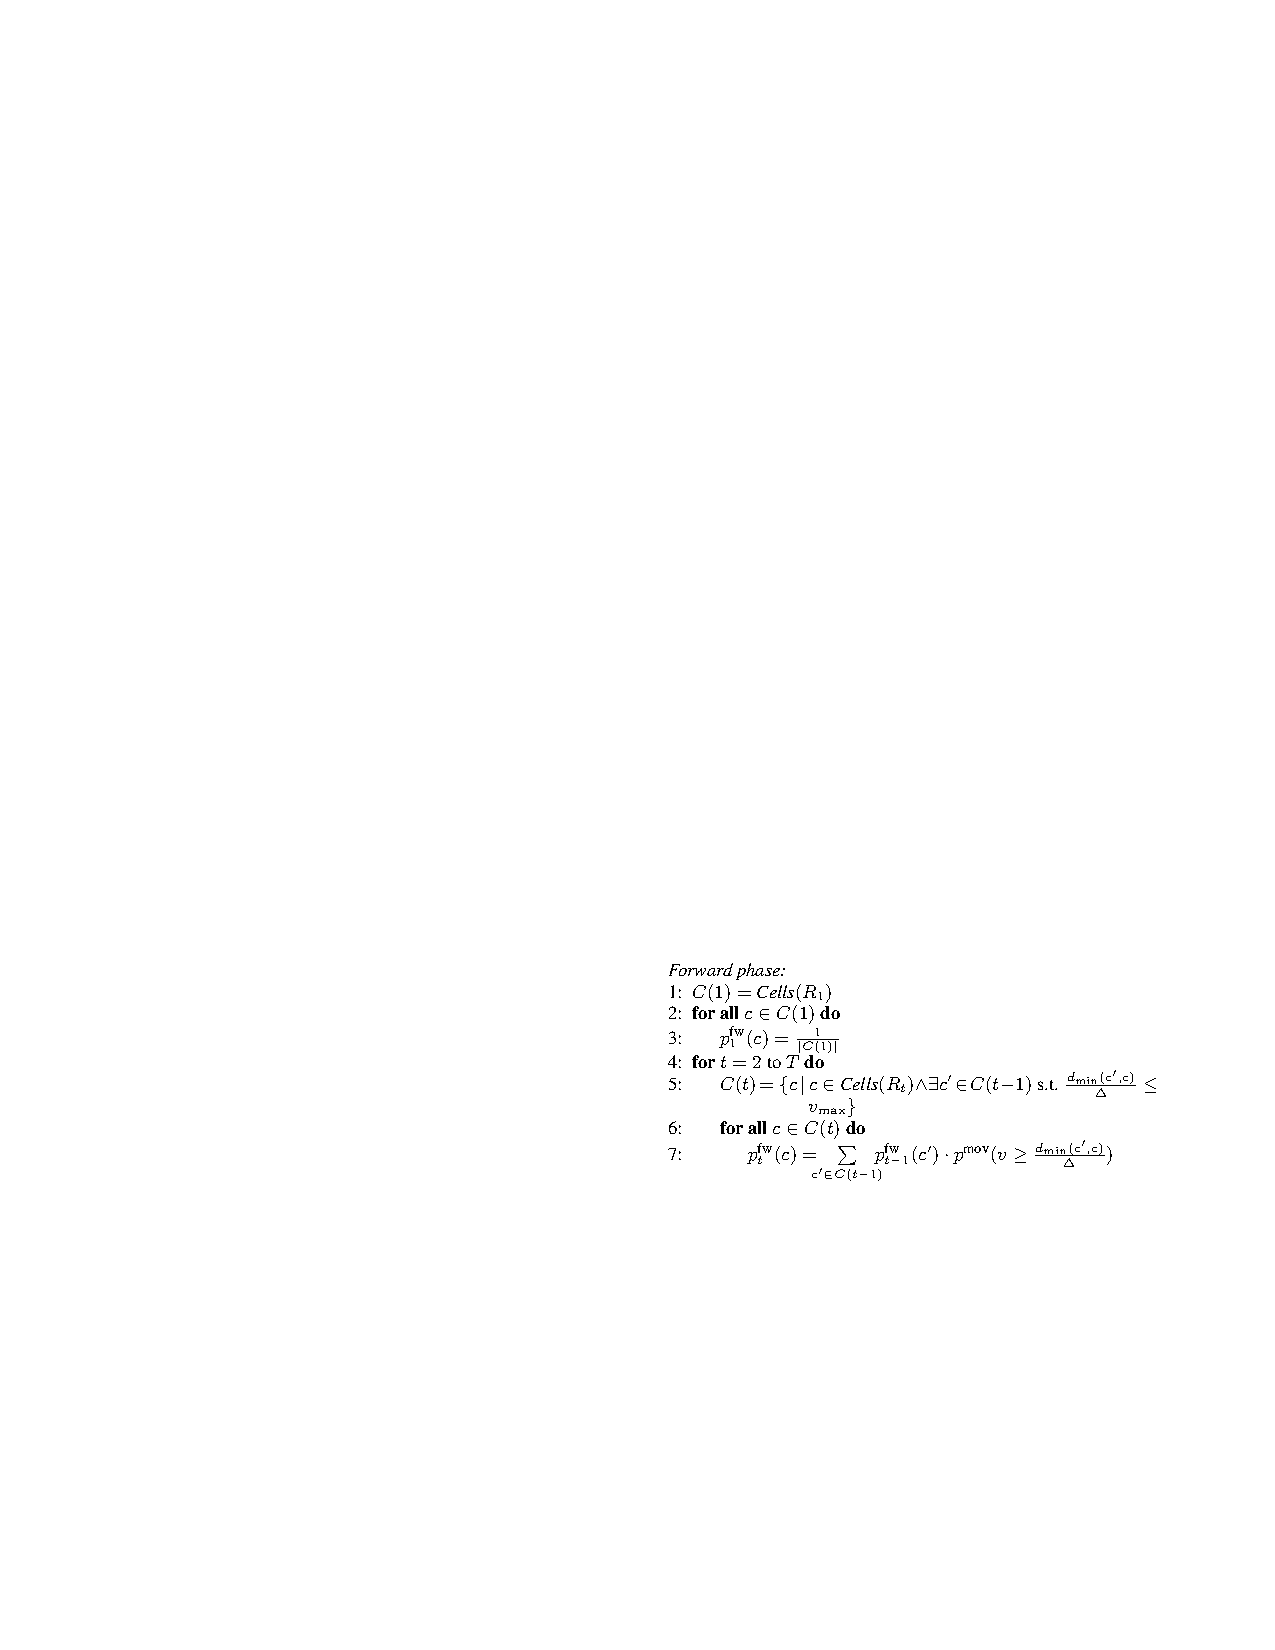
\includegraphics[width=\columnwidth]{figures/3-4/3-4-22.pdf}
\end{figure}

\column{0.45\textwidth}
\ssize{
\begin{enumerate}
  \item lines 1--3: $C(1)$ is assigned the set of the cells in $Cells(R_1)$, while $p^{fw}_t$ is assumed uniformly distributed.
  \item lines 4--7: for each time point $t$ in $[2...T]$, $C(t)$ is evaluated as the set of cells of $Cells(R_t)$ which are reachable by at least one cell $c' \in C(t-1)$ in one time unit, considering the movement limitations implied by the map and the maximum speed.
\end{enumerate}
}

\end{columns}

\end{frame}

%------------------------------------------------

\begin{frame}
\frametitle{Exhaustive Approach: Forward Phase}

\begin{columns}

\column{0.4\textwidth}
\begin{figure}[tb]
  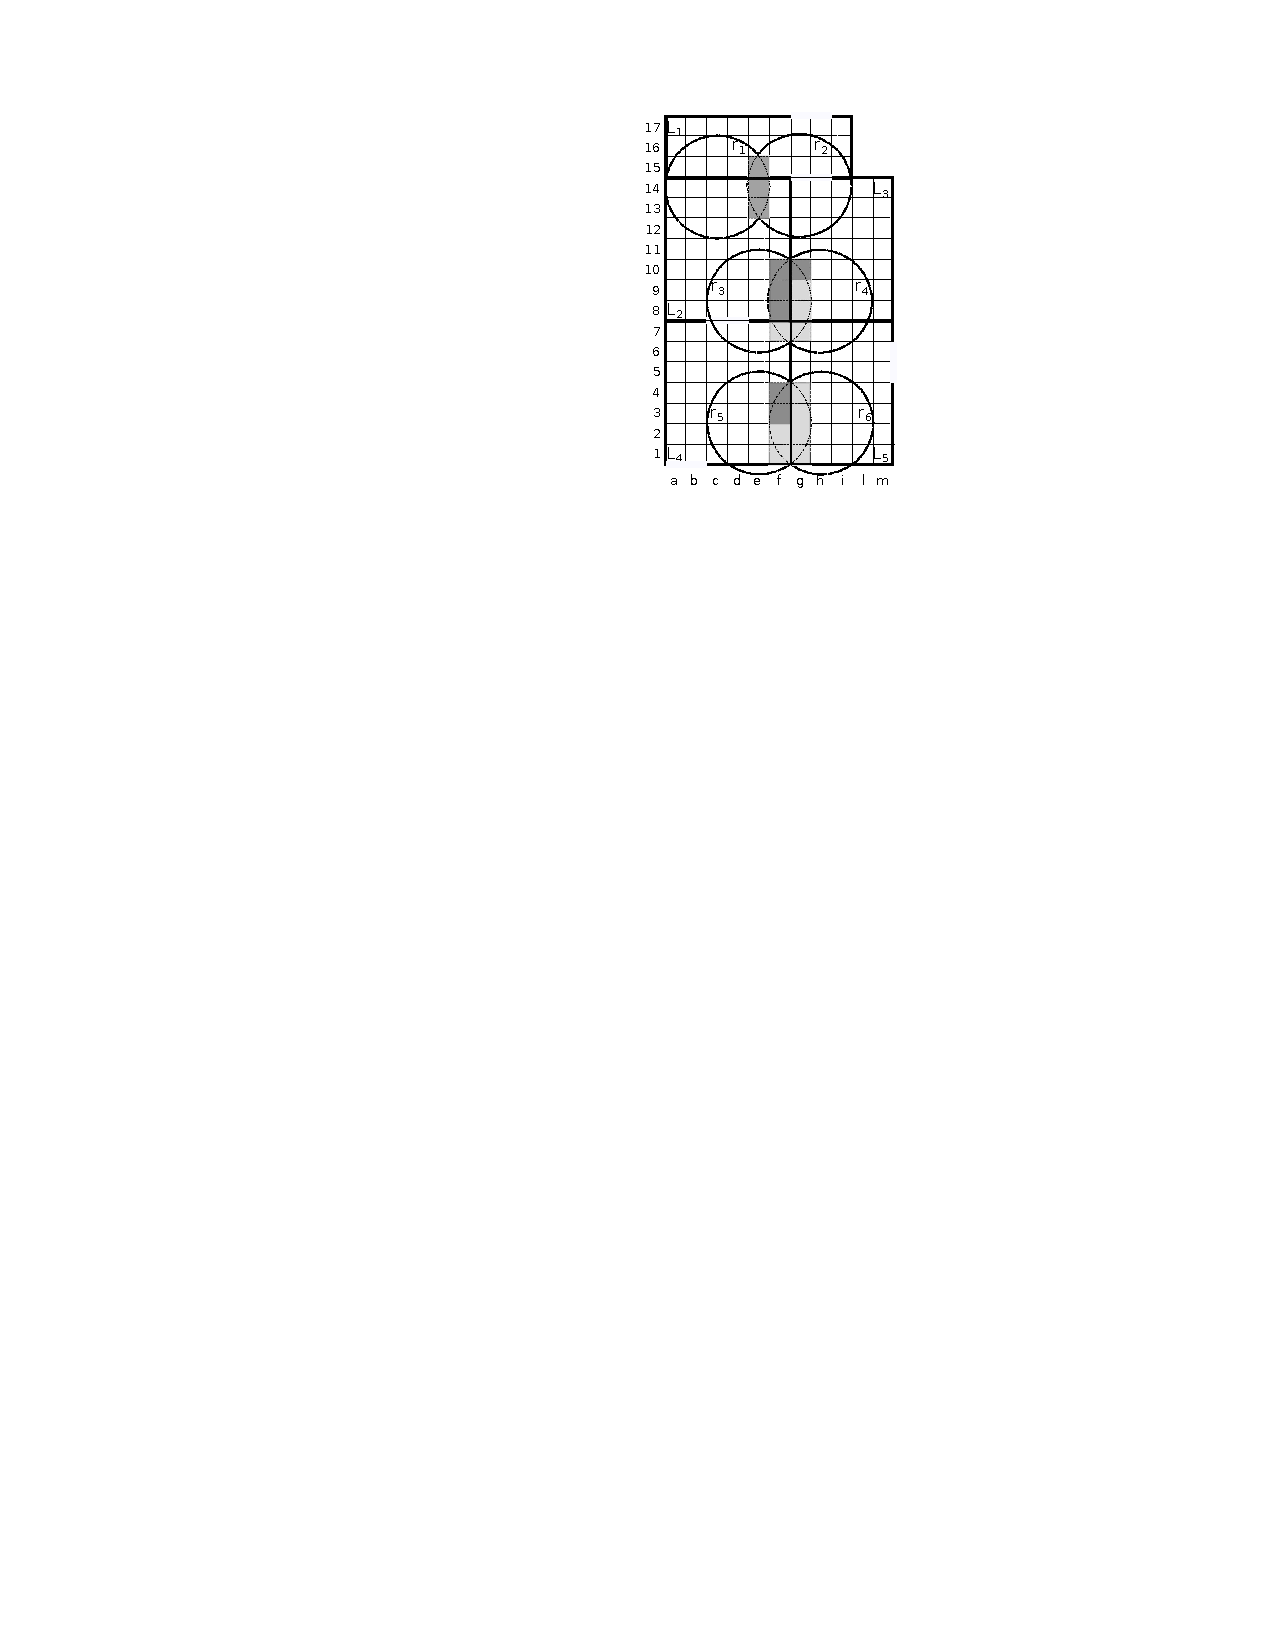
\includegraphics[width=\columnwidth]{figures/3-4/3-4-17.pdf}
\end{figure}

\column{0.6\textwidth}
\begin{figure}[tb]
  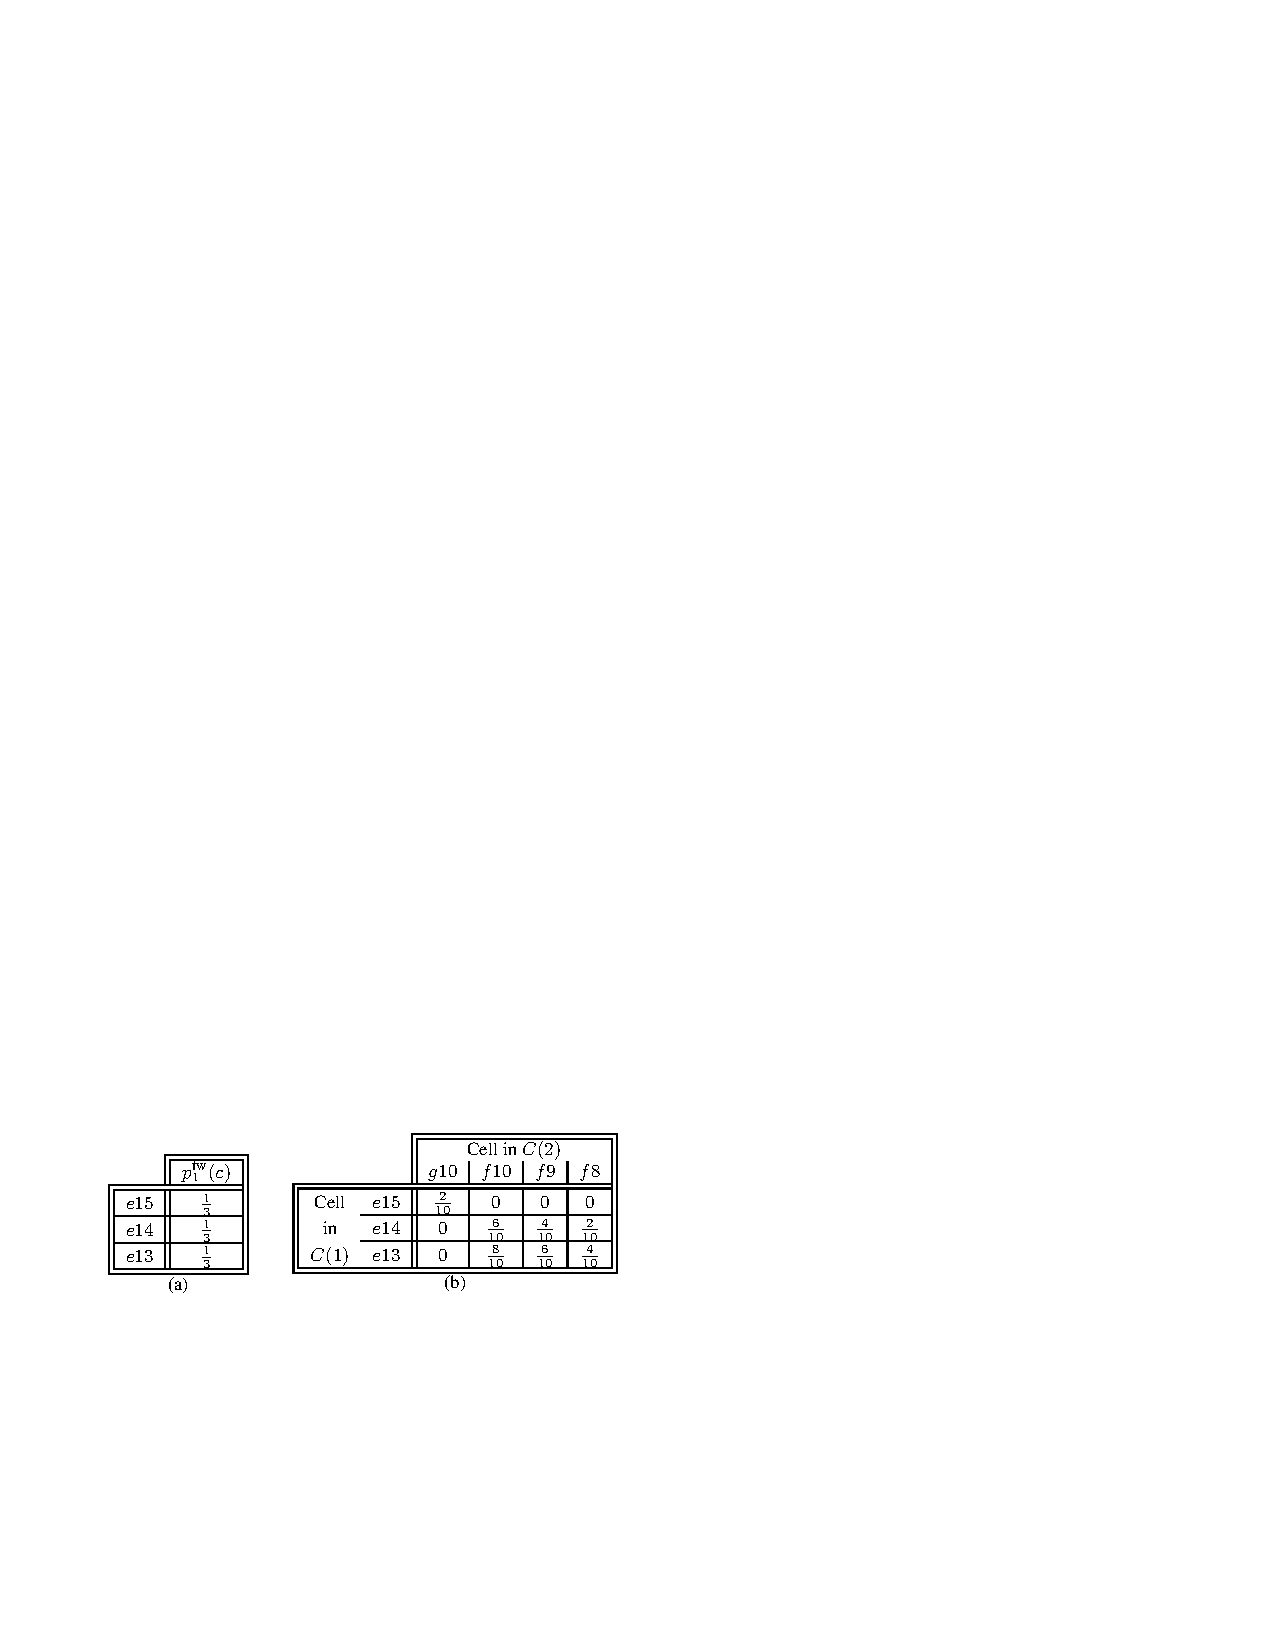
\includegraphics[width=\columnwidth]{figures/3-4/3-4-18.pdf}
\end{figure}

\ssize{

\textbf{STEP I-1}\quad set $C(1) = Cells(R_1) = \{ e13,e14,e15 \}$, assign probability $p^{fw}_1(c) = \frac{1}{3}$ to each cell $c \in C(1)$.\\~\\

\textbf{STEP I-2}\quad At $t = 2$, $Cells(R_2) = \{ f7,f8,f9,f10,g7,g8,g9,g10 \}$. Among these cells, only the dark-gray colored ones are reachable in one time unit. I.e., cells $f8,f9,f10,g10$ are reachable from $e13$ and $e14$, while cell $g10$ is reachable from $e15$. The $p^{mov}$ is computed as figure(b).

}

\end{columns}

\end{frame}

%------------------------------------------------

\begin{frame}
\frametitle{Exhaustive Approach: Forward Phase}

\begin{columns}

\column{0.4\textwidth}
\begin{figure}[tb]
  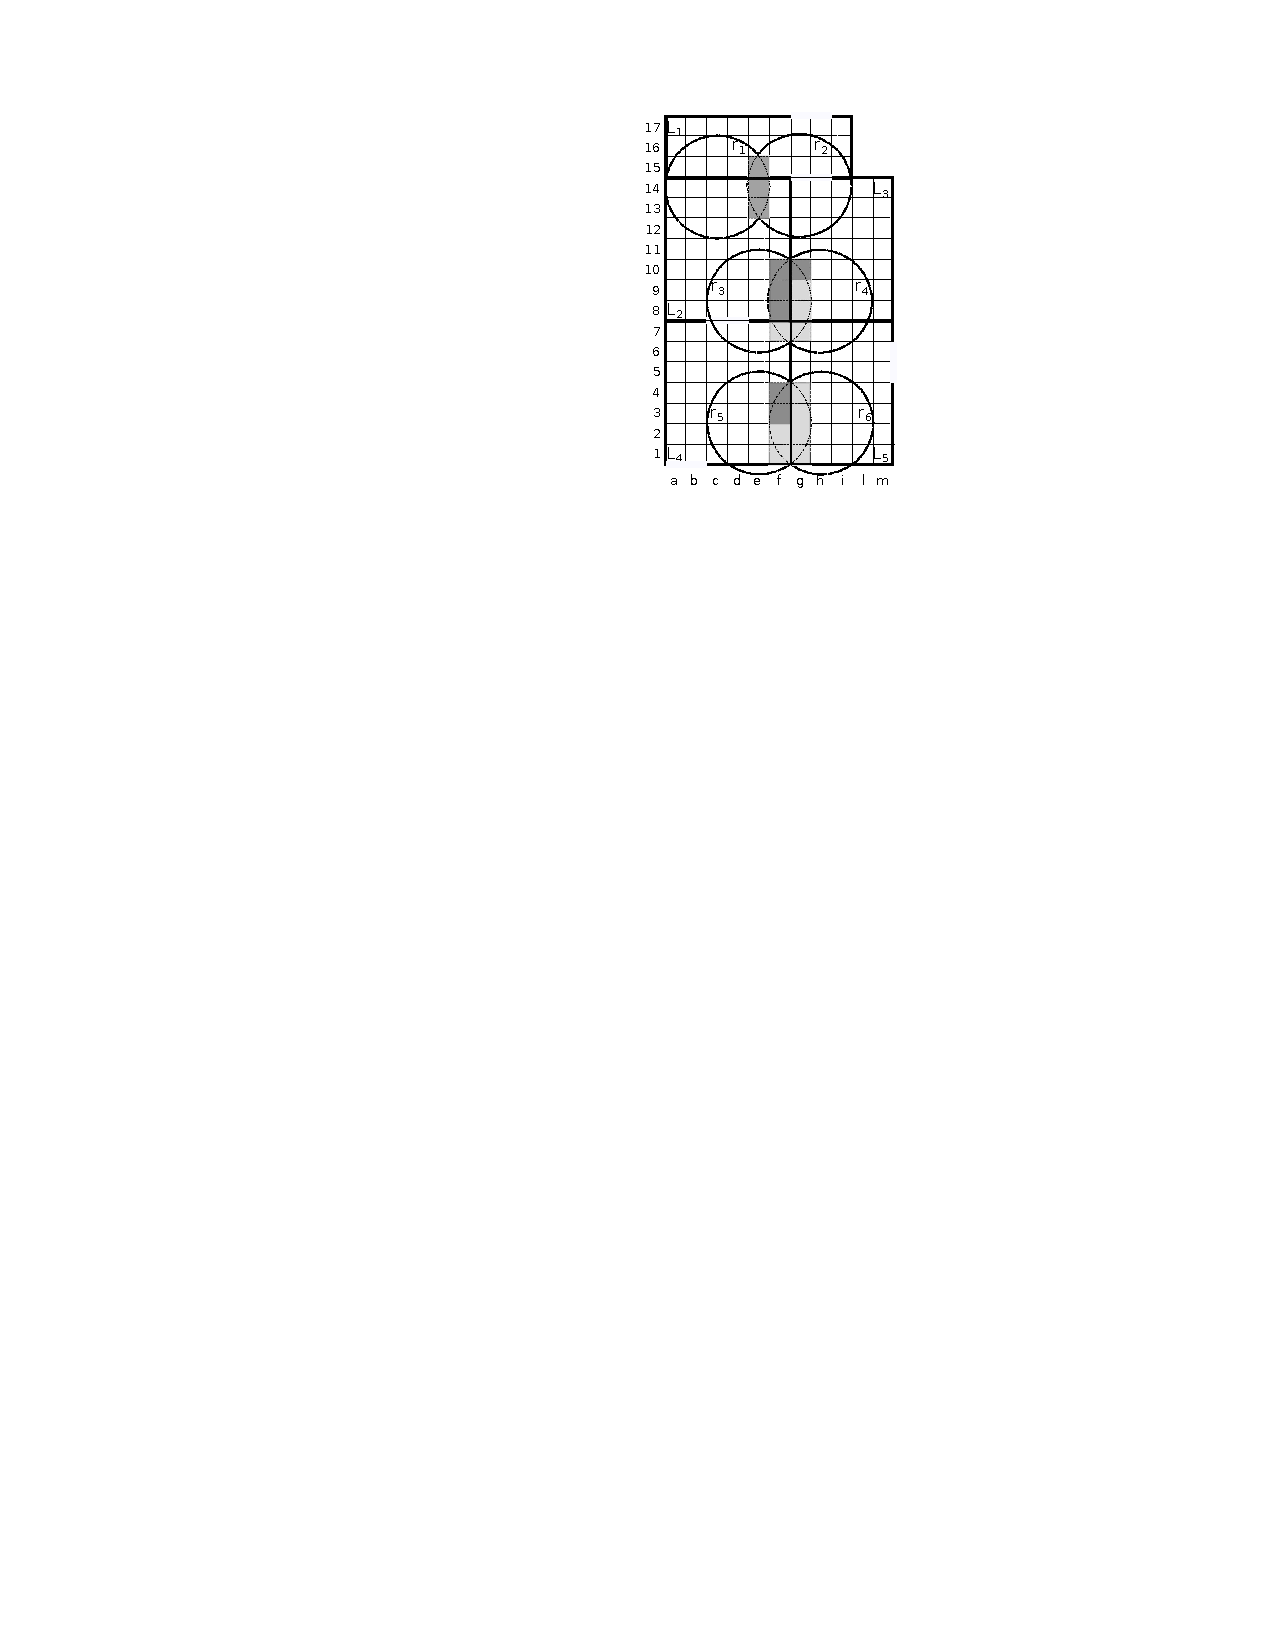
\includegraphics[width=\columnwidth]{figures/3-4/3-4-17.pdf}
\end{figure}

\column{0.6\textwidth}
\begin{figure}[tb]
  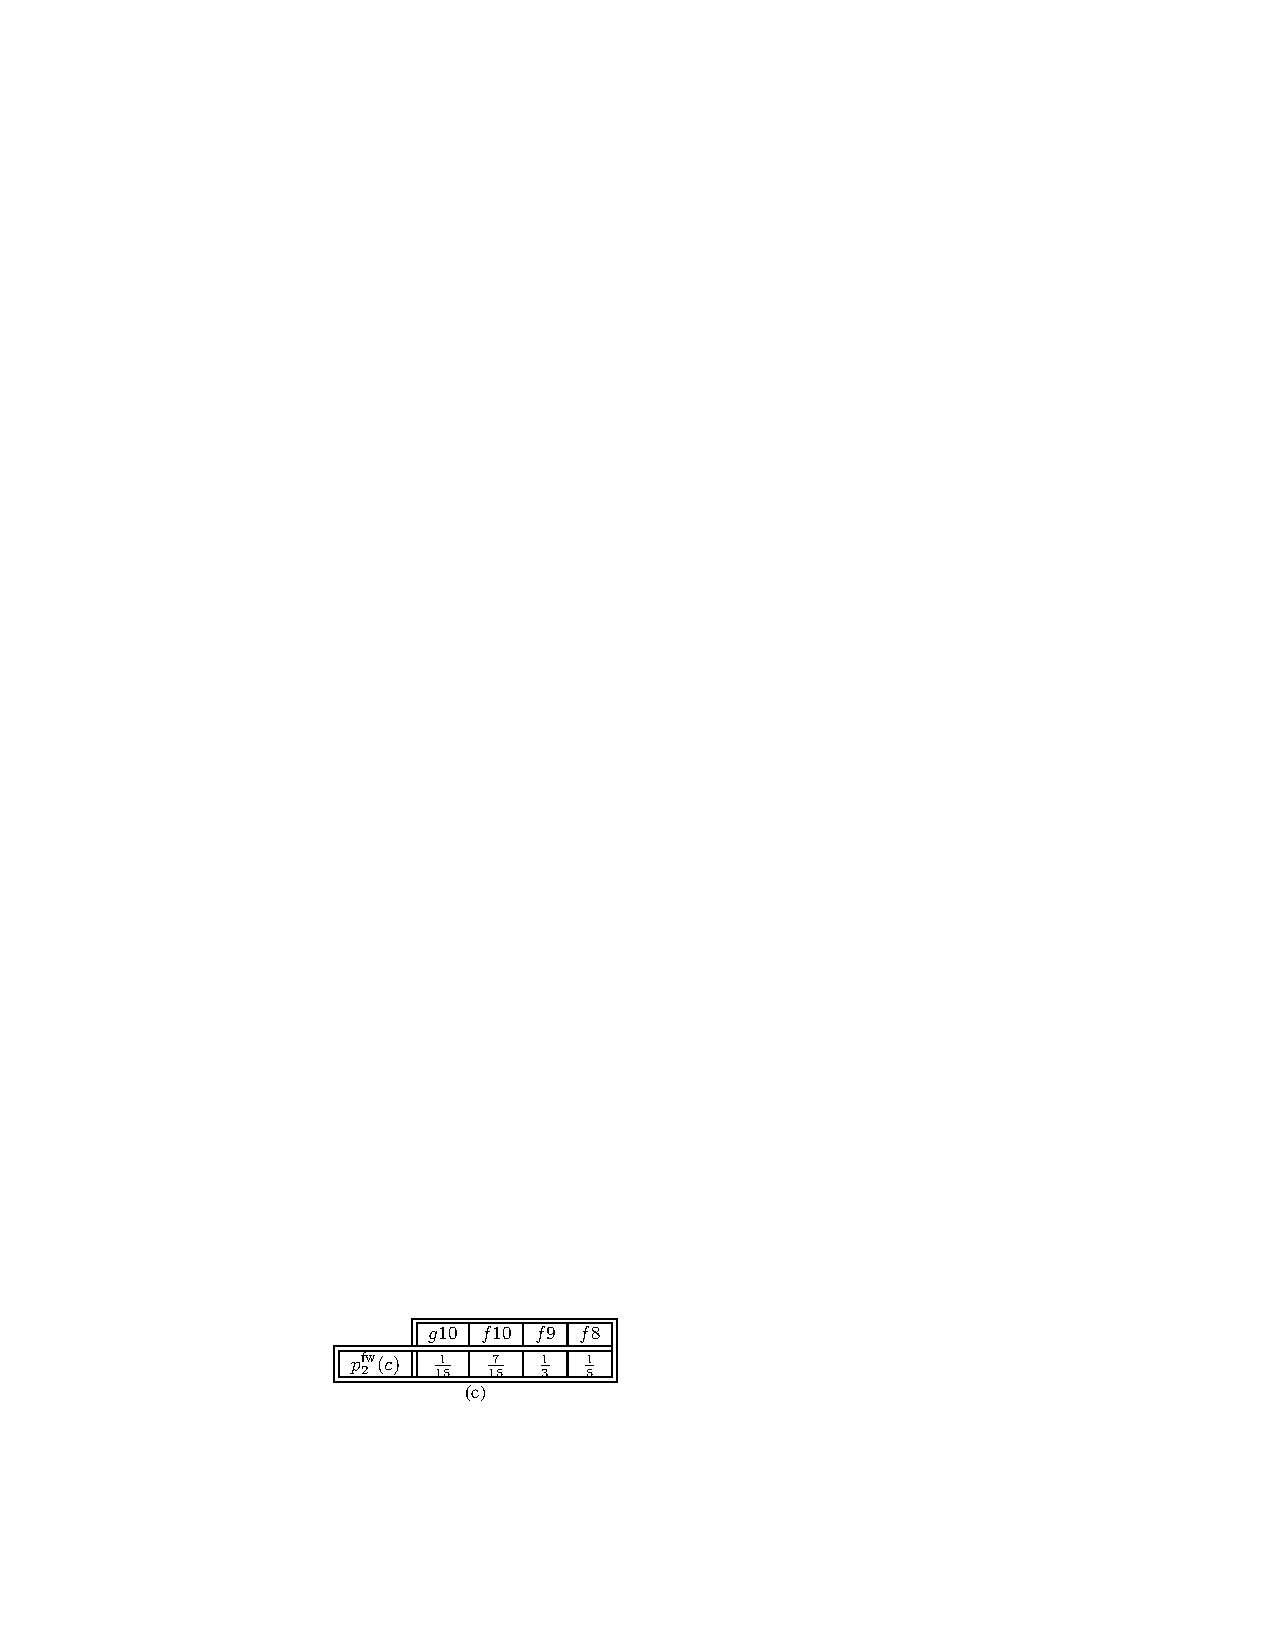
\includegraphics[width=\columnwidth]{figures/3-4/3-4-19.pdf}
\end{figure}

\ssize{

\textbf{STEP I-3}\quad the forward probability shown in figure(c) is obtained by summing the products of forward probabilities of cell $c_i$ shown in figure(a) with the corresponding $p^{mov}$ in figure(b). For instance, $p^{fw}_2(f10) = \frac{1}{3} \cdot 0 + \frac{1}{3} \cdot \frac{6}{10} + \frac{1}{3} \cdot \frac{8}{10} = \frac{7}{15}$.
}

\end{columns}

\end{frame}

%------------------------------------------------

\begin{frame}
\frametitle{Exhaustive Approach: Forward Phase}

\begin{columns}

\column{0.4\textwidth}
\begin{figure}[tb]
  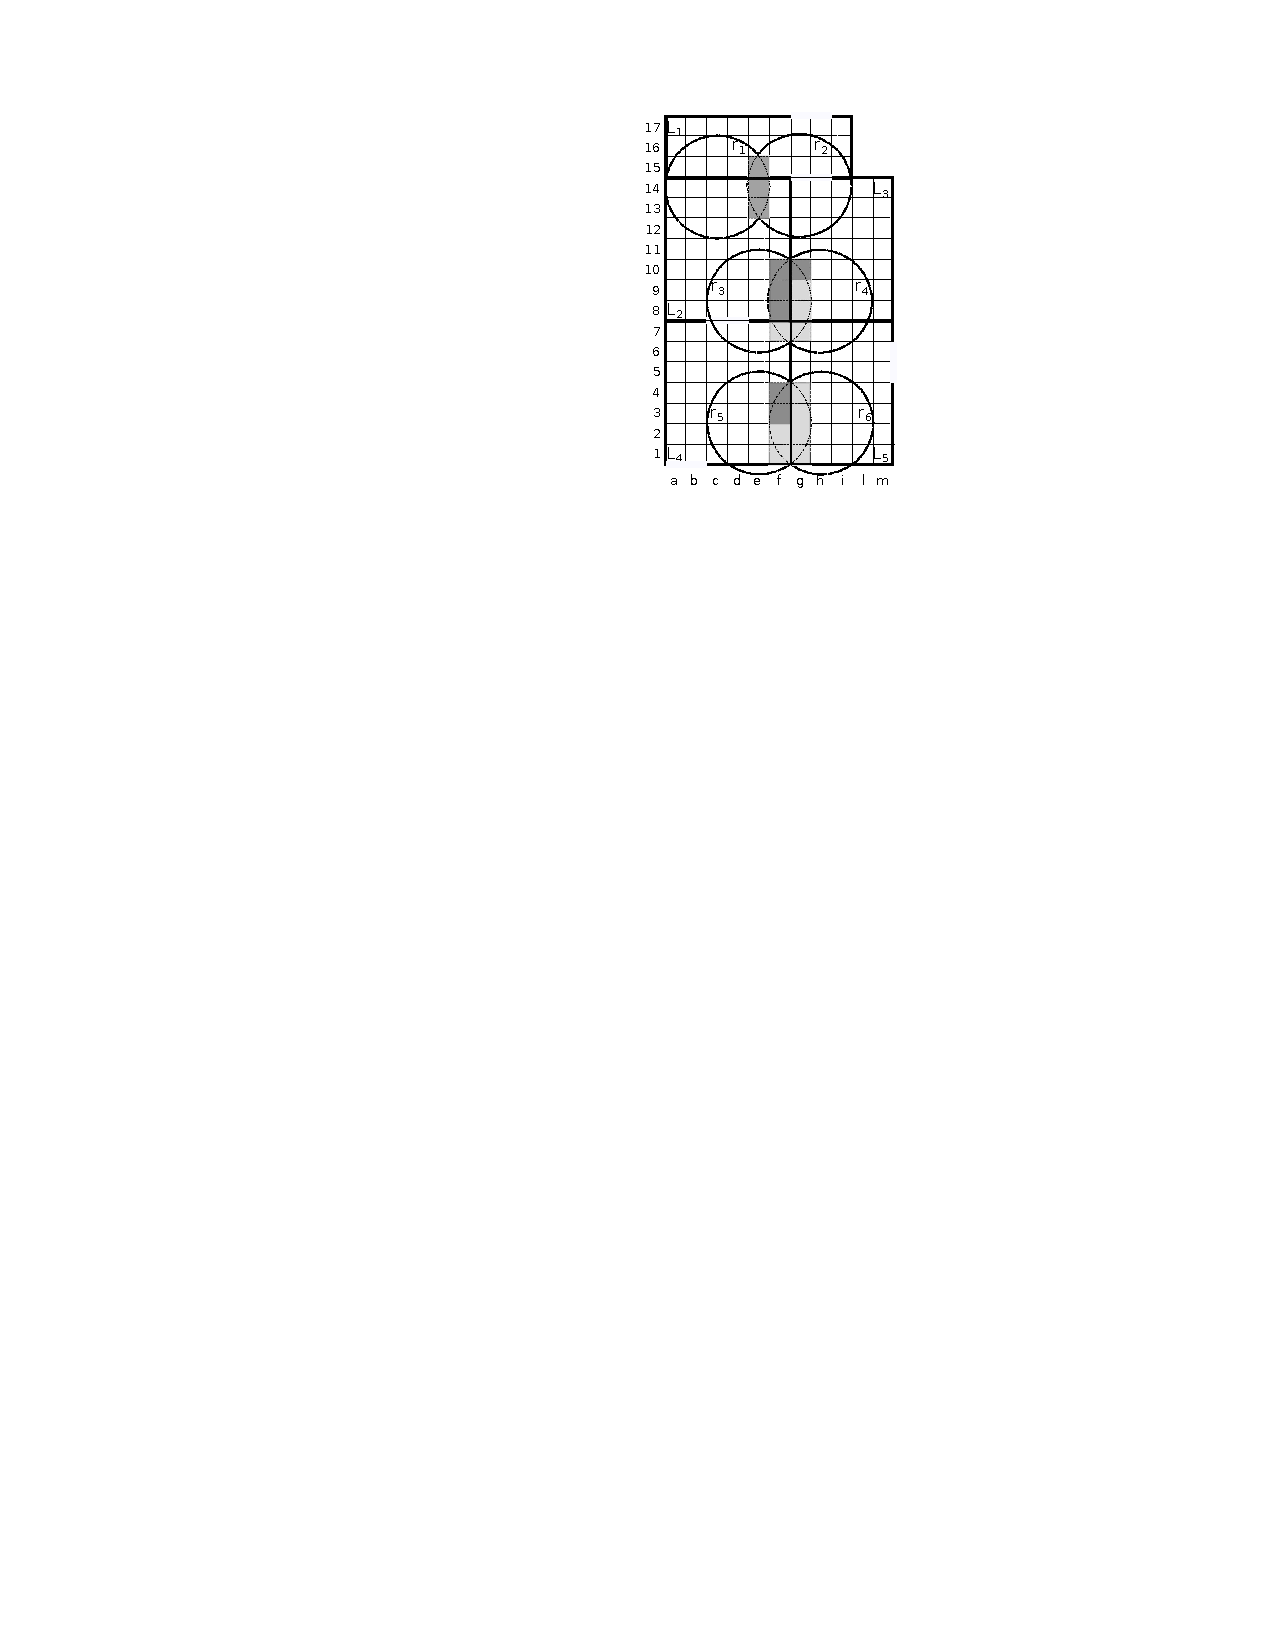
\includegraphics[width=\columnwidth]{figures/3-4/3-4-17.pdf}
\end{figure}

\column{0.6\textwidth}
\begin{figure}[tb]
  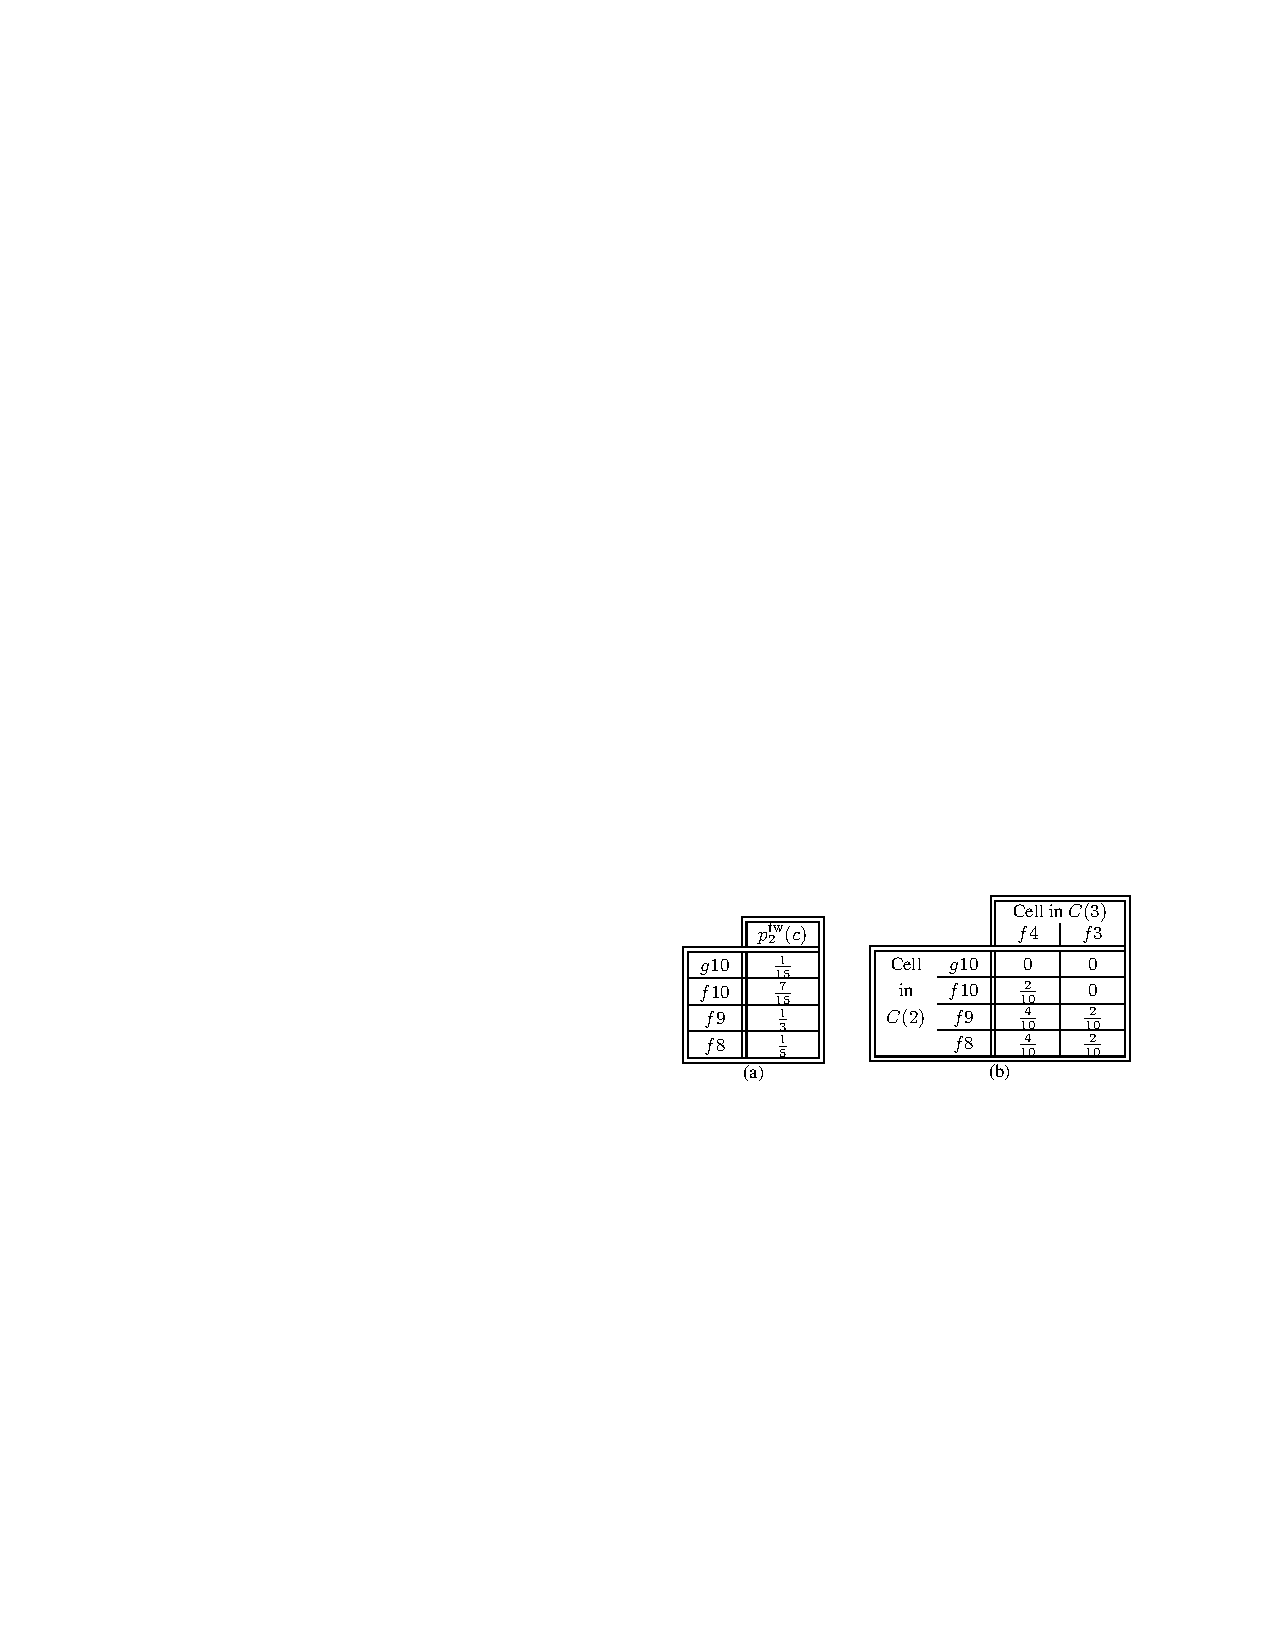
\includegraphics[width=\columnwidth]{figures/3-4/3-4-20.pdf}
\end{figure}

\ssize{

\textbf{STEP II-1}\quad from $\{ g10,f10,f9,f8 \}$ shown in figure(a), only $\{ f4,f3,f2,f1 \}$ can be reached while $\{ g4,g3,g2,g1 \}$ cannot.\\~\\

\textbf{STEP II-2}\quad only the dark-grayed cells $C(3) = \{ f3,f4 \}$ can meet the maximum speed condition, the $p^{mov}(v \geq \frac{d_{min}(c_i,c_j)}{\Delta})$ are computed in figure(b).
}

\end{columns}

\end{frame}

%------------------------------------------------

\begin{frame}
\frametitle{Exhaustive Approach: Forward Phase}

\begin{columns}

\column{0.4\textwidth}
\begin{figure}[tb]
  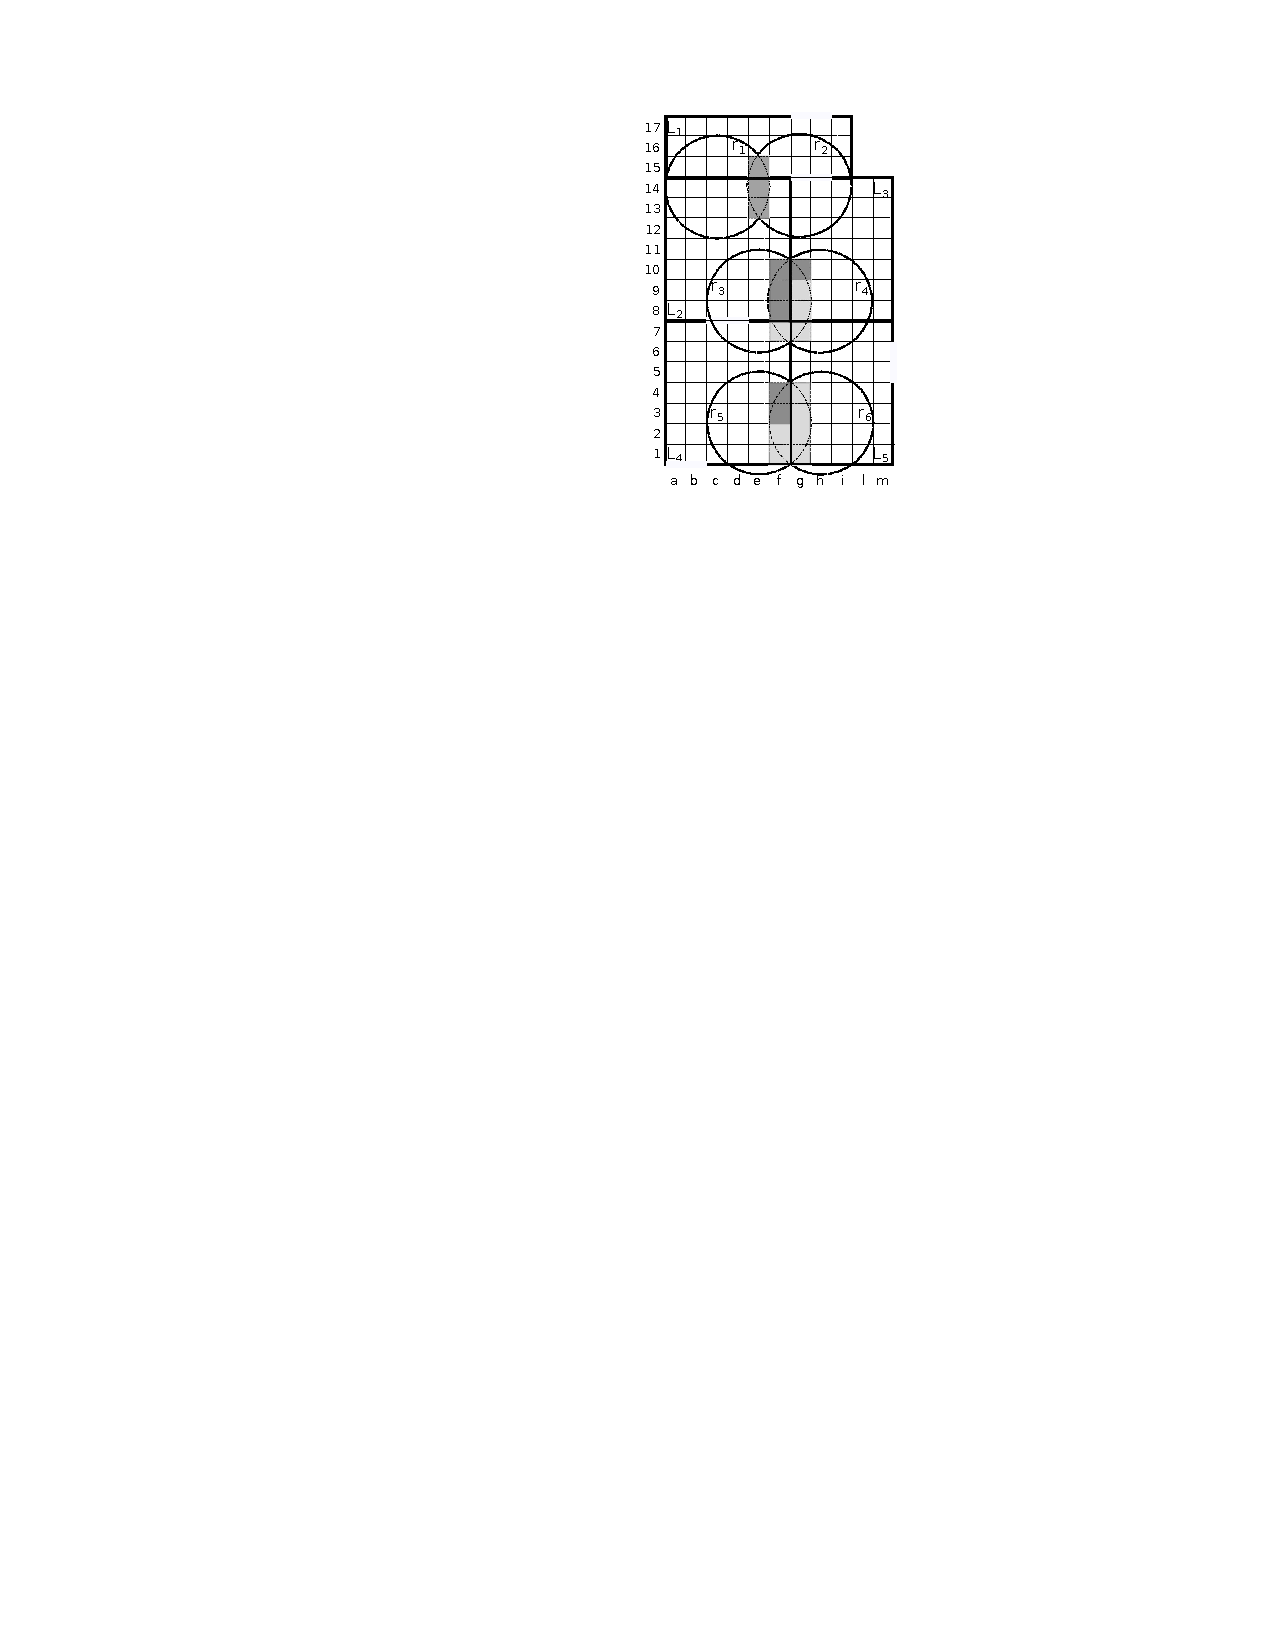
\includegraphics[width=\columnwidth]{figures/3-4/3-4-17.pdf}
\end{figure}

\column{0.6\textwidth}
\begin{figure}[tb]
  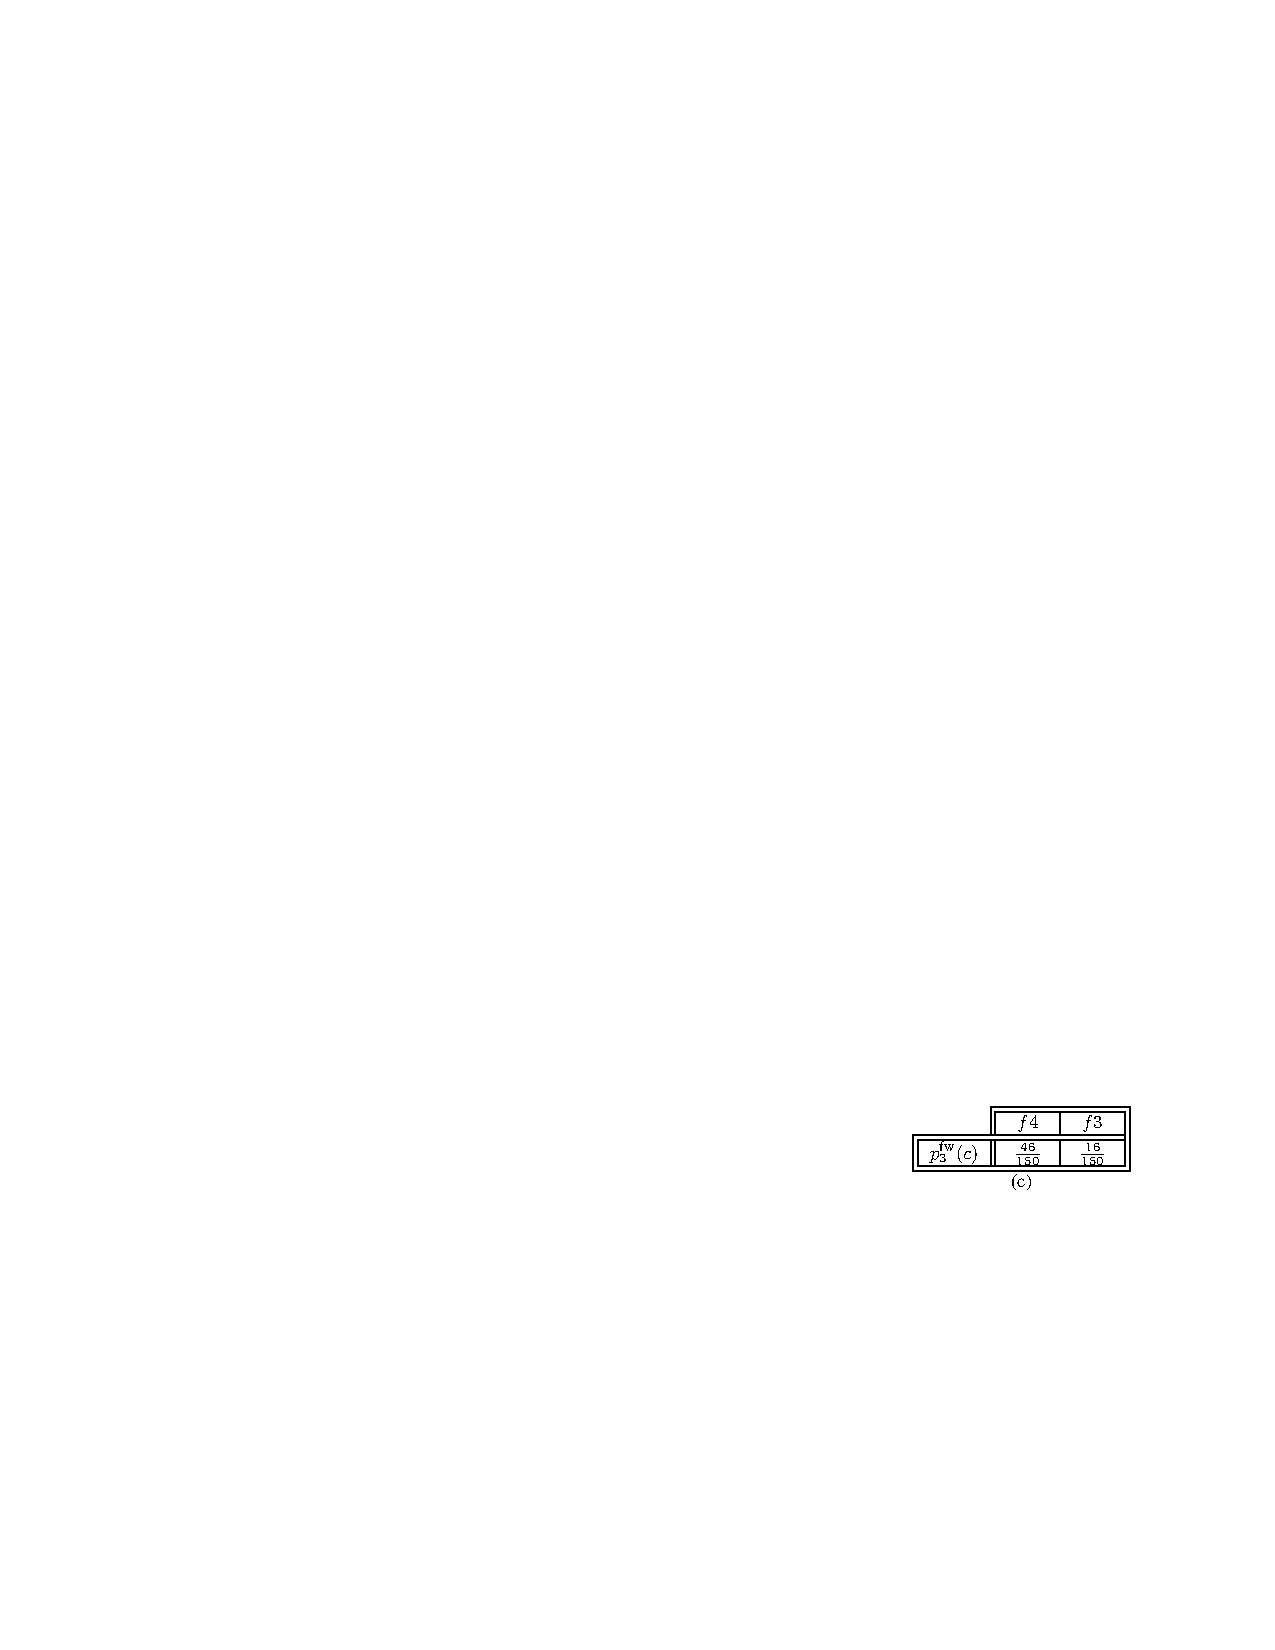
\includegraphics[width=\columnwidth]{figures/3-4/3-4-21.pdf}
\end{figure}

\ssize{

\textbf{STEP II-3}\quad the forward probability shown in figure(c) is obtained by summing the products of forward probabilities of cell $c_i$ shown in figure(a) with the corresponding $p^{mov}$ in figure(b). For instance, $p^{fw}_3(f4) = \frac{1}{15} \cdot 0 + \frac{7}{15} \cdot \frac{2}{10} + \frac{1}{3} \cdot \frac{4}{10} + \frac{1}{5} \cdot \frac{4}{10} = \frac{46}{150}$.
}

\end{columns}

\end{frame}

%------------------------------------------------

\begin{frame}
\frametitle{Exhaustive Approach: Backward Phase and Final Steps}

\begin{columns}

\column{0.5\textwidth}
\begin{figure}[tb]
  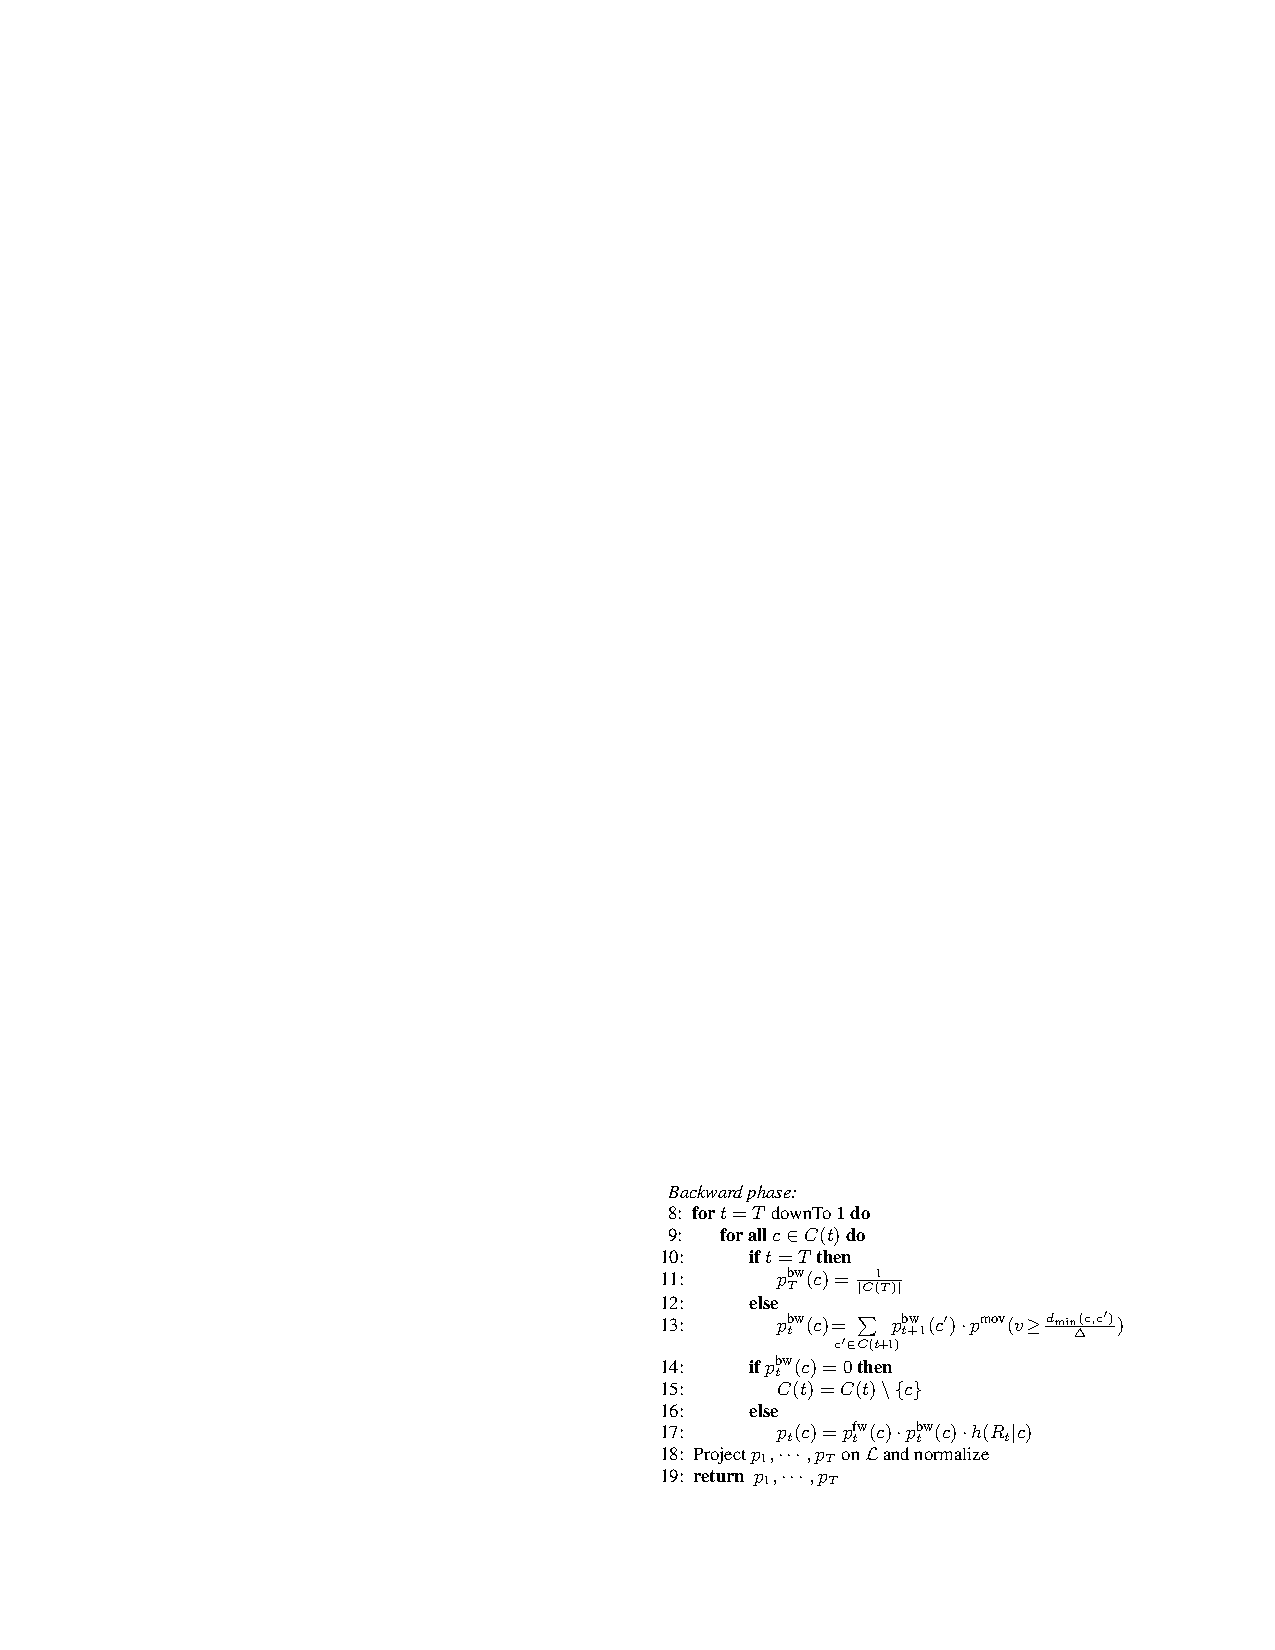
\includegraphics[width=\columnwidth]{figures/3-4/3-4-23.pdf}
\end{figure}

\column{0.5\textwidth}
\ssize{
\begin{enumerate}
  \item line 11: scan the time points in $[1...T]$ in inverse order, and assigns uniform probability $p^{bw}_T$ to the cells in $C(T)$.
  \item line 15: if a cell has backward probability equal to 0, it's removed from $C(t)$, since it is incompatible with the future positions.
  \item line 17: the algorithm computes the probability $p_t(c)$ by multiplying the backward probability with the forward probablity resulting from the forward phase and the likelihood $h(R_t|c)$.
  \item line 18: the so obtained probabilities are projected on $\mathcal{L}$, fianlly, these probabilities are normalized, and the p-trajectories are returned.
\end{enumerate}
}

\end{columns}

\end{frame}

%------------------------------------------------

\begin{frame}
\frametitle{Exhaustive Approach: Backward Phase and Final Steps}

\begin{columns}

\column{0.4\textwidth}
\begin{figure}[tb]
  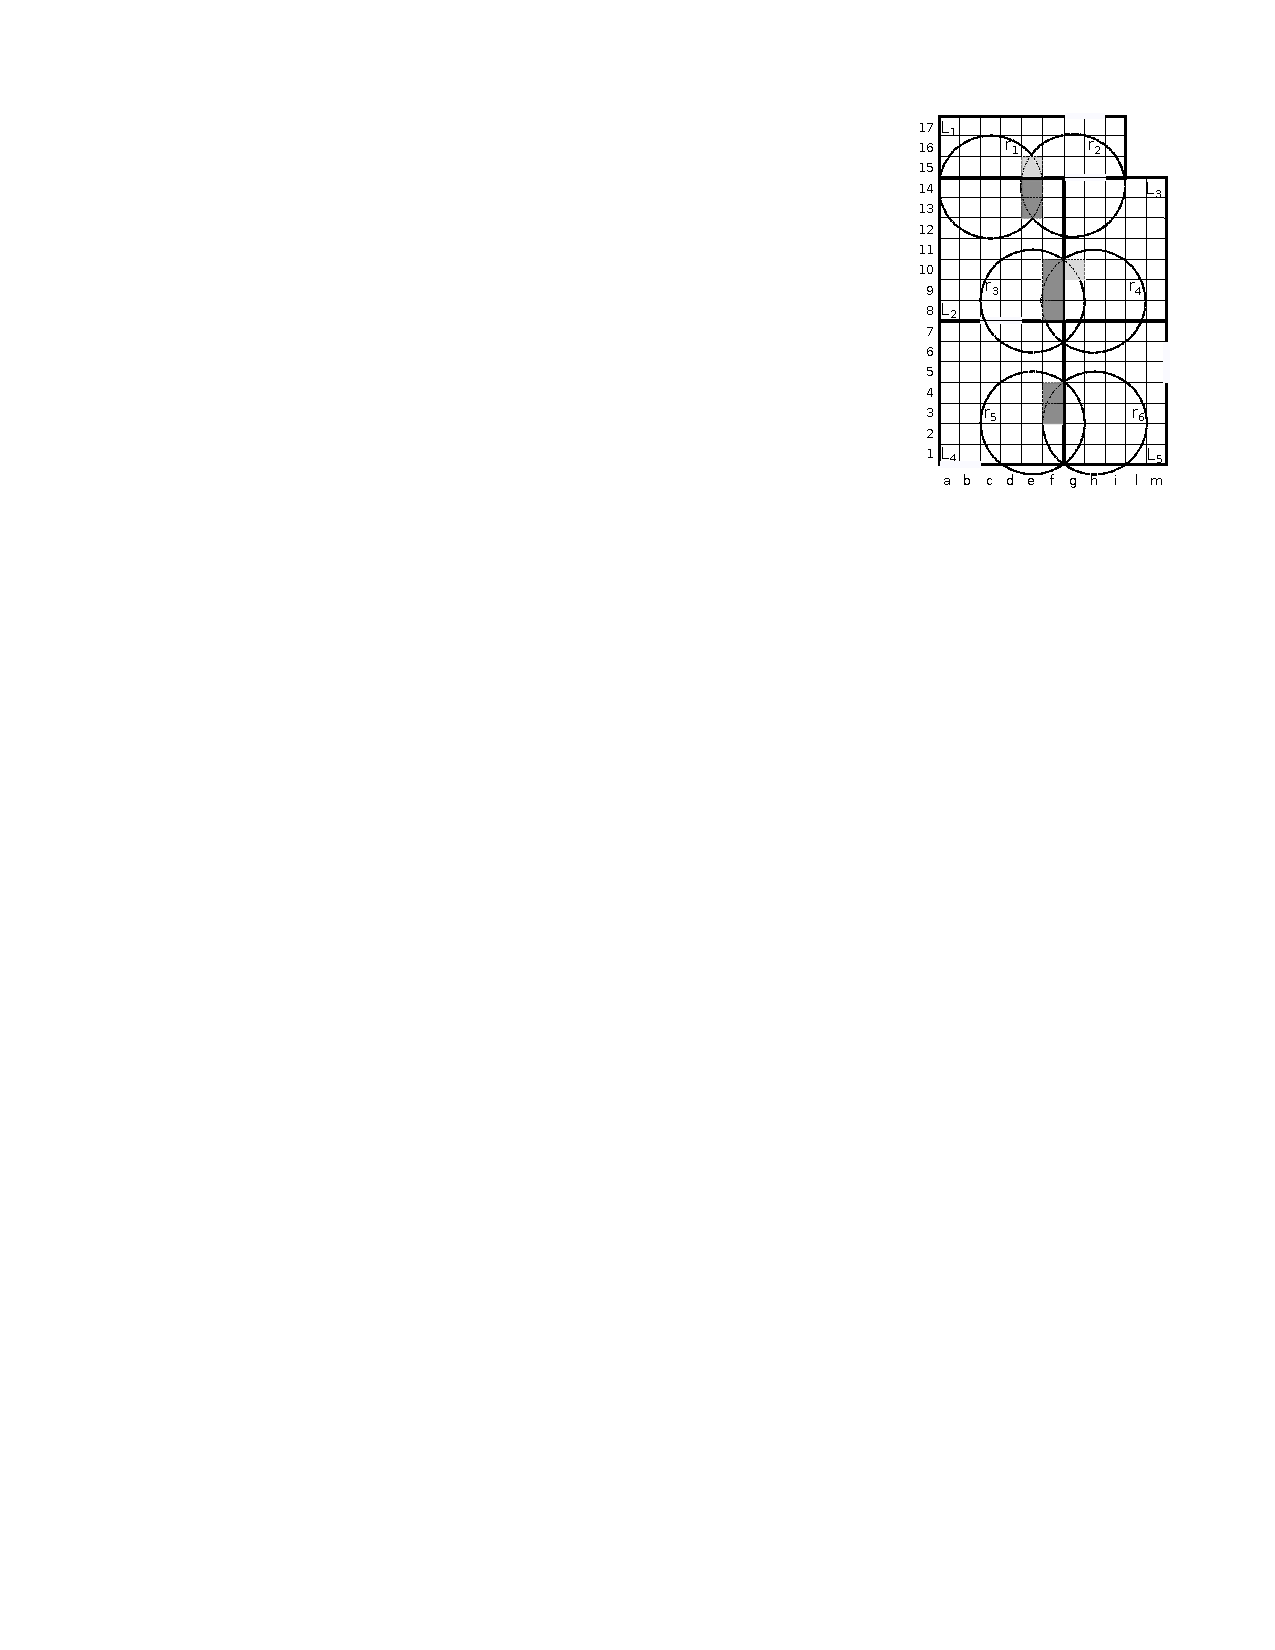
\includegraphics[width=\columnwidth]{figures/3-4/3-4-24.pdf}
\end{figure}

\column{0.6\textwidth}

\ssize{

\textbf{STEP III-1}\quad assigns $p^{bw}_3(c) = \frac{1}{2}$ for each of the two cells in $C(3)$.\\~\\

\textbf{STEP III-2}\quad $p^{bw}_2(g10) = 0$ (remove it), $p^{bw}_2(f10) = \frac{1}{2} \cdot \frac{2}{10} = \frac{1}{10}$, $p^{bw}_2(f9) = \frac{1}{2} \cdot \frac{6}{10} = \frac{3}{10}$, $p^{bw}_2(f8) = \frac{1}{2} \cdot \frac{6}{10} = \frac{3}{10}$.\\~\\

\textbf{STEP III-3}\quad $p^{bw}_3(e14) = \frac{1}{10} \cdot \frac{6}{10} + \frac{3}{10} \cdot \frac{4}{10} + \frac{3}{10} \cdot \frac{2}{10} = \frac{24}{100}$, $p^{bw}_3(e13) = \frac{1}{10} \cdot \frac{8}{10} + \frac{3}{10} \cdot \frac{6}{10} + \frac{3}{10} \cdot \frac{4}{10} = \frac{38}{100}$.\\~\\

\textbf{STEP III-4}\quad the posterior probability $p_t(c)$ is computed by projection: $p_1(L_2) = p_1(e13) + p_1(e14)$, $p_2(L_2) = p_2(f10) + p_2(f9) + p_2(f8)$, $p_3(L_4) = p_3(f4) + p_3(f3)$. After normalization, the probabilities that $o$ was at location $L_2$ at time points 1 and 2, and at $L_4$ at time 3 are $100\%$.

}

\end{columns}

\end{frame}

%------------------------------------------------

\begin{frame}
\frametitle{Exhaustive Approach: Unsuitability for Missing Detections}

\begin{block}{}
  \ssize{
  $C(t)$ is the set of cells with two properties:

  \begin{itemize}
    \item i. they are covered by the set $R_t$;
    \item ii. they are reachable in one time unit from at least a cell in $C(t-1)$ without exceeding the speed limit imposed by $v_{max}$.
  \end{itemize}

  In the case of missing detection (i.e., $R_t = \varnothing$) , the size of $C(t)$ strongly depends on the maximum speed and the size of $C(t-1)$.
  }
\end{block}

Even if $C(t-1)$ and $v_{max}$ are such that the size of $C(t)$ is smaller than the number of cells covered by one reader, it is easy to see that, in the presence of a sequence of $m$ missing detections starting at time $t$, the size of $C(t+m)$ may become extremely large.

\end{frame}

%------------------------------------------------

% \begin{frame}
% \frametitle{Sampling-based Approach}
%
%
%
% \end{frame}
